\documentclass[../AISTR.tex]{subfiles}

\begin{document}
\section{ПО для моделирования нанесения покрытия}
\subsection{Краткое резюме}\label{par:resume}
Описанное ниже программное обеспечение является учебным и позволяет смоделировать нанесение покрытия на внутреннюю часть тонкой цилиндрической трубки, расположенной под наклоном методом Монте-Карло.

Программа генерирует случайные числа (в данном случае случайным числом является синус угла распыления). 

Для записи результатов применяется словарь (число-структура).
Ключ словаря -- нижнее значение интервала разбиения длины трубки. Например, если молекула попала на отрезок $\left[10, 20\right]$, то ключём будет $10$. 

Значением является структура \textit{values} (см. листинг \rbf{list:map}). Структура содержит в себе поле значения количества попавших в интервал молекул, а также координаты каждой из молекул по стороне $L$.



\begin{lstlisting}[caption=Запись значений,captionpos=b, label={list:map}]
	struct value
	{
		int i;
		vector<double> vec;
	};
	map<int, value> right_values;
	map<int, value> left_values;
\end{lstlisting}

Программа совершает большое количество итераций по описанному далее методу и выводит результаты в файл (см. листинг \rbf{list:file}). В файле содержится количество попавших в каждый интервал на каждой стороне молекул. 
\subsection{Расчёт геометрии}\label{par:geom}
\subsubsection{Эскиз}
На \refris{fig:eskiz} изображён эскиз будущего расчёта. 
\begin{enumerate}
	\item Трубка, на внутреннюю поверхность которой наносятся частицы;
	\item Точечный источник, из которого вылетают частицы;
	\item Частицы.
\end{enumerate}
\begin{figure}
	\centering
	%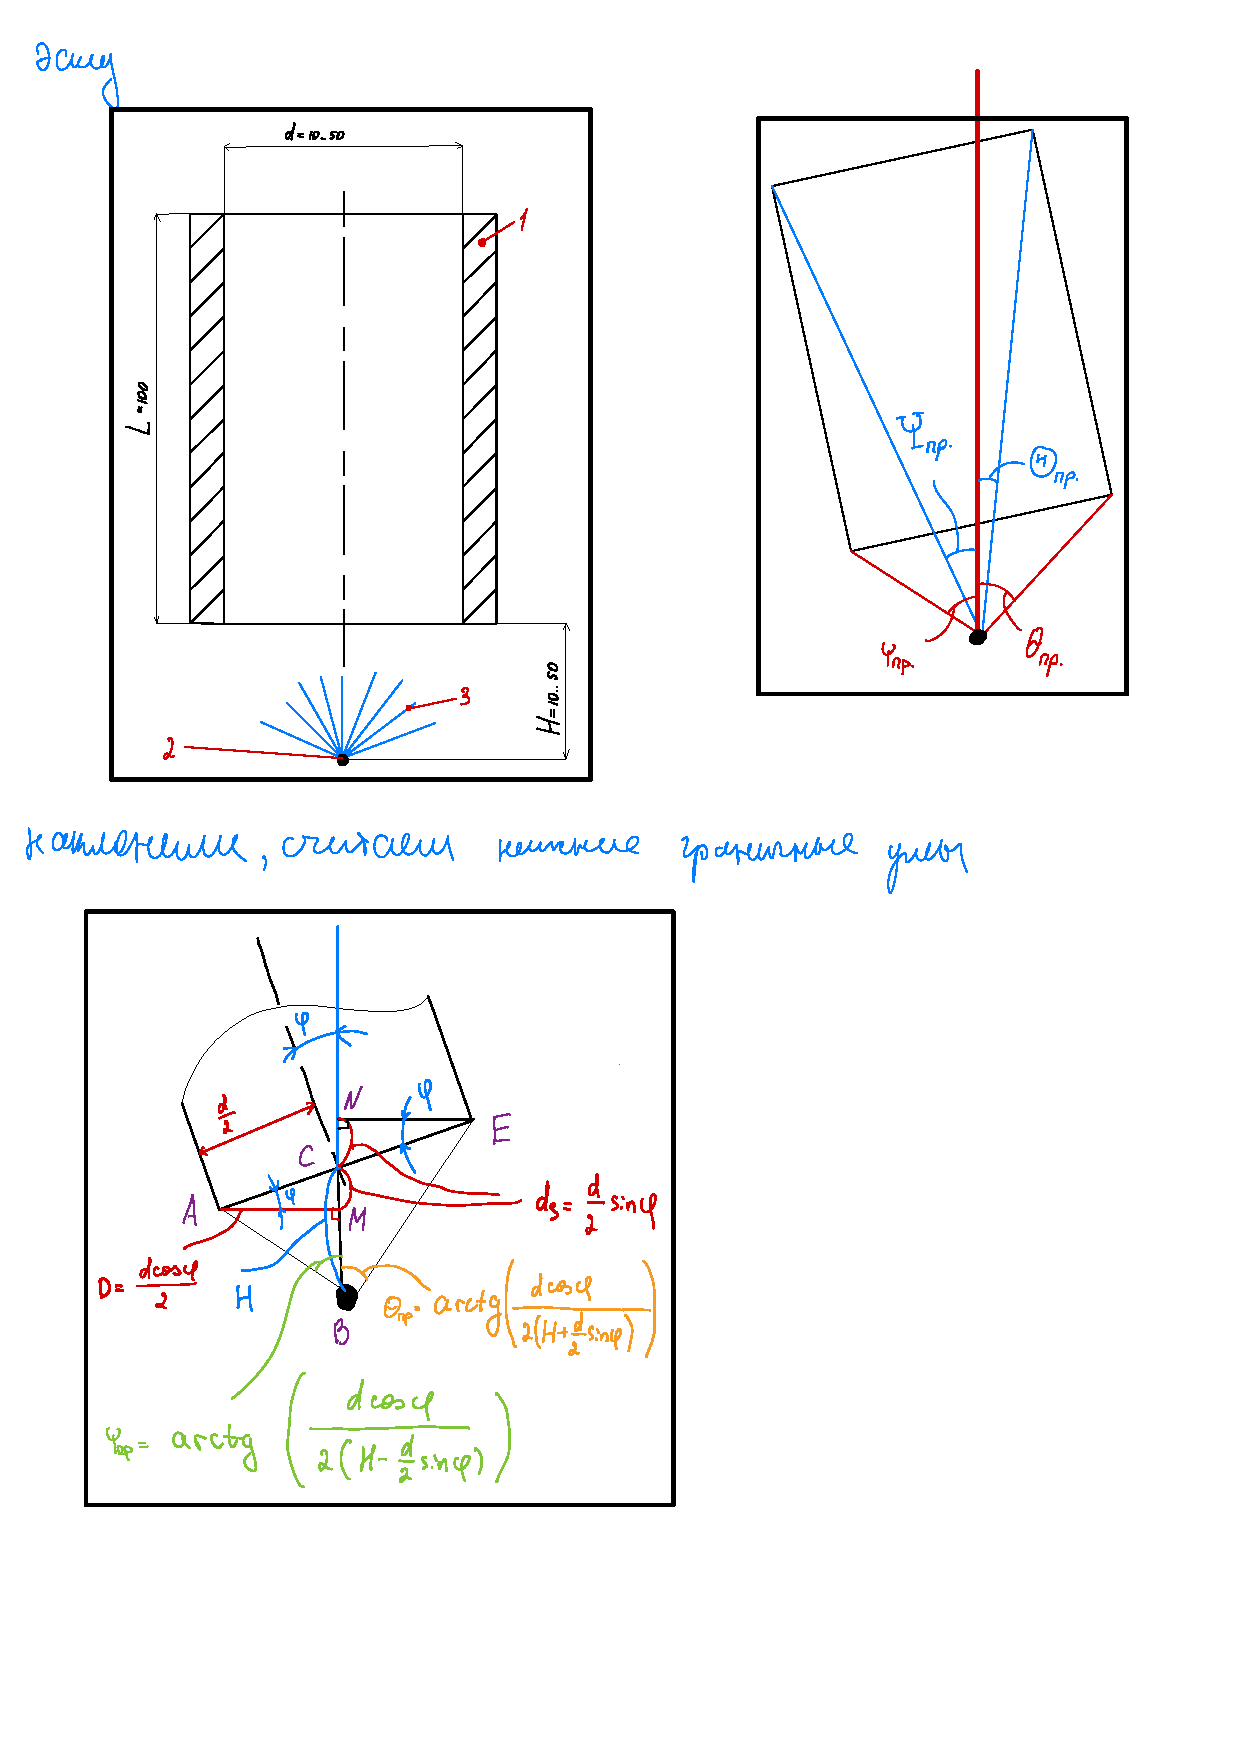
\includegraphics[trim=60 470 320 60, clip, width=0.5\linewidth]{../images/t1}
	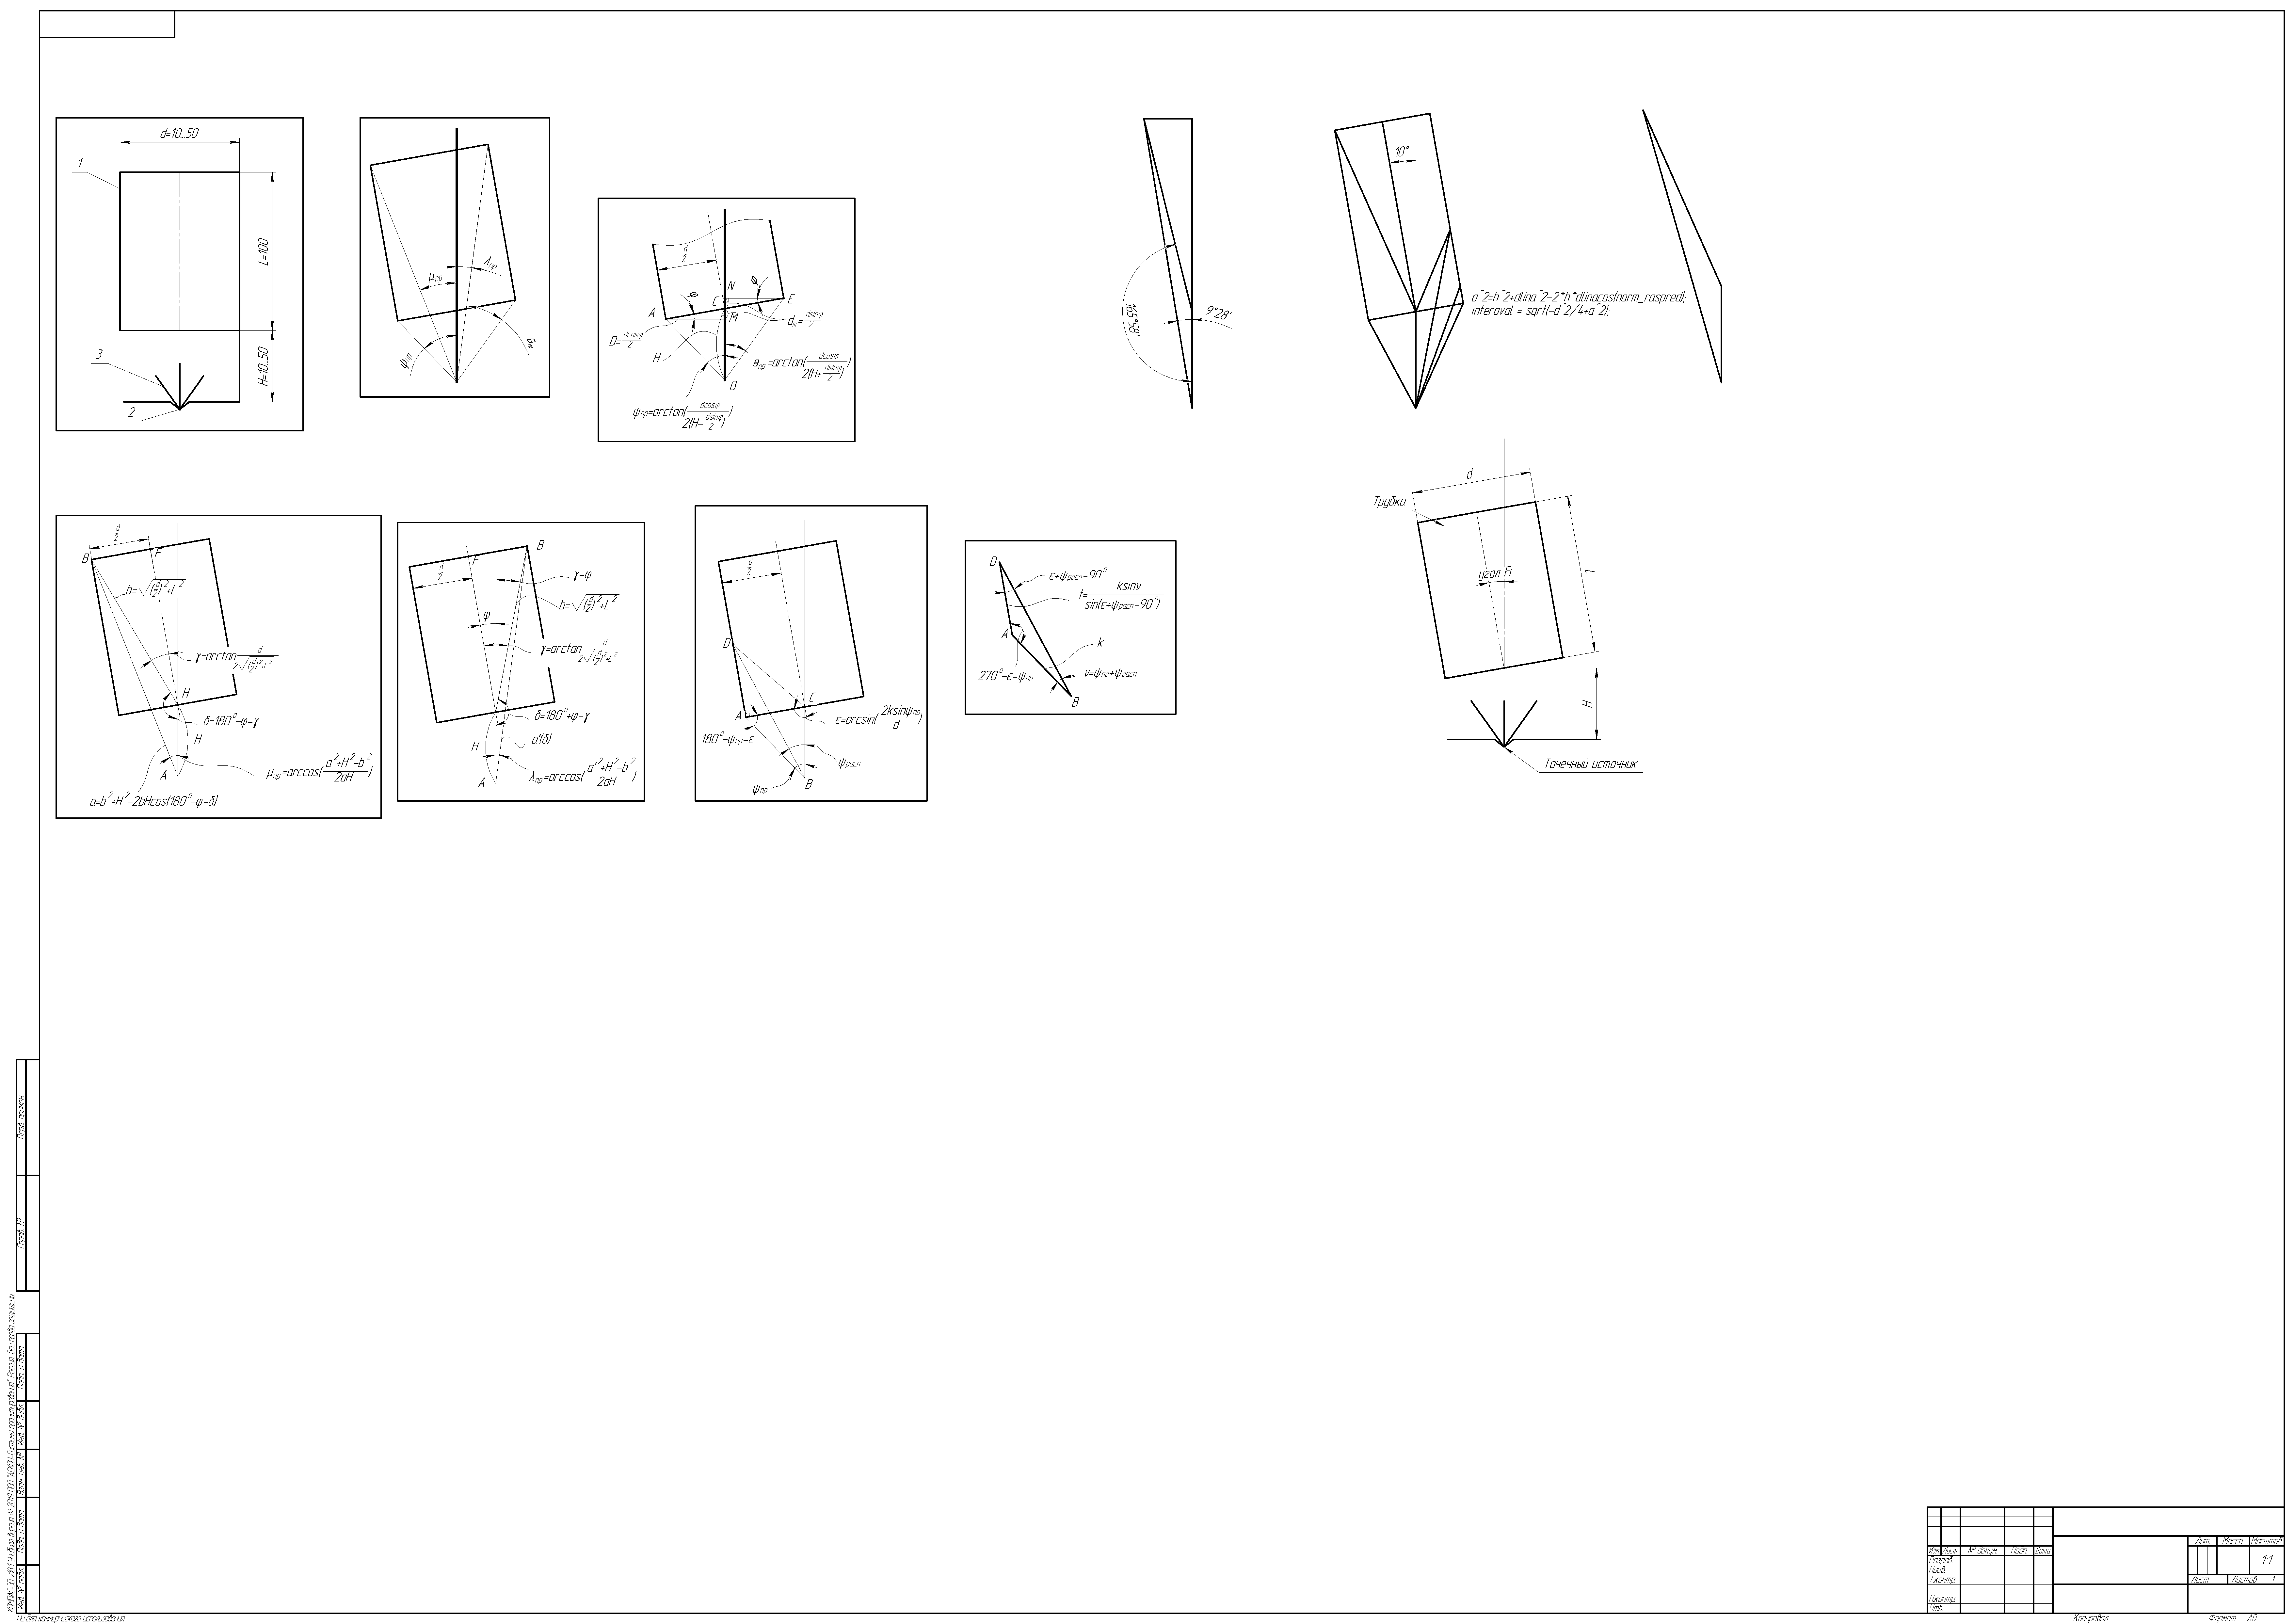
\includegraphics[trim=85 1765 2940 180, clip, width=0.5\linewidth]{../images/schemes}
	\caption{Экскиз расчёта}
	\label{fig:eskiz}
\end{figure}
\subsubsection{Граничные условия}
Молекулы будут попадать на внутреннюю поверхность в том случае, если (см. \refris{fig:border}):
\begin{itemize}
	\item \textbf{слева:} угол распыления
	\begin{equation}
		\fr \in \left[\lu, \ld\right]
	\end{equation}
	\item \textbf{справа:} угол распыления
	\begin{equation}
		\fr \in \left[\ru, \rd\right]
	\end{equation}
\end{itemize}


\begin{figure}
	\centering
	%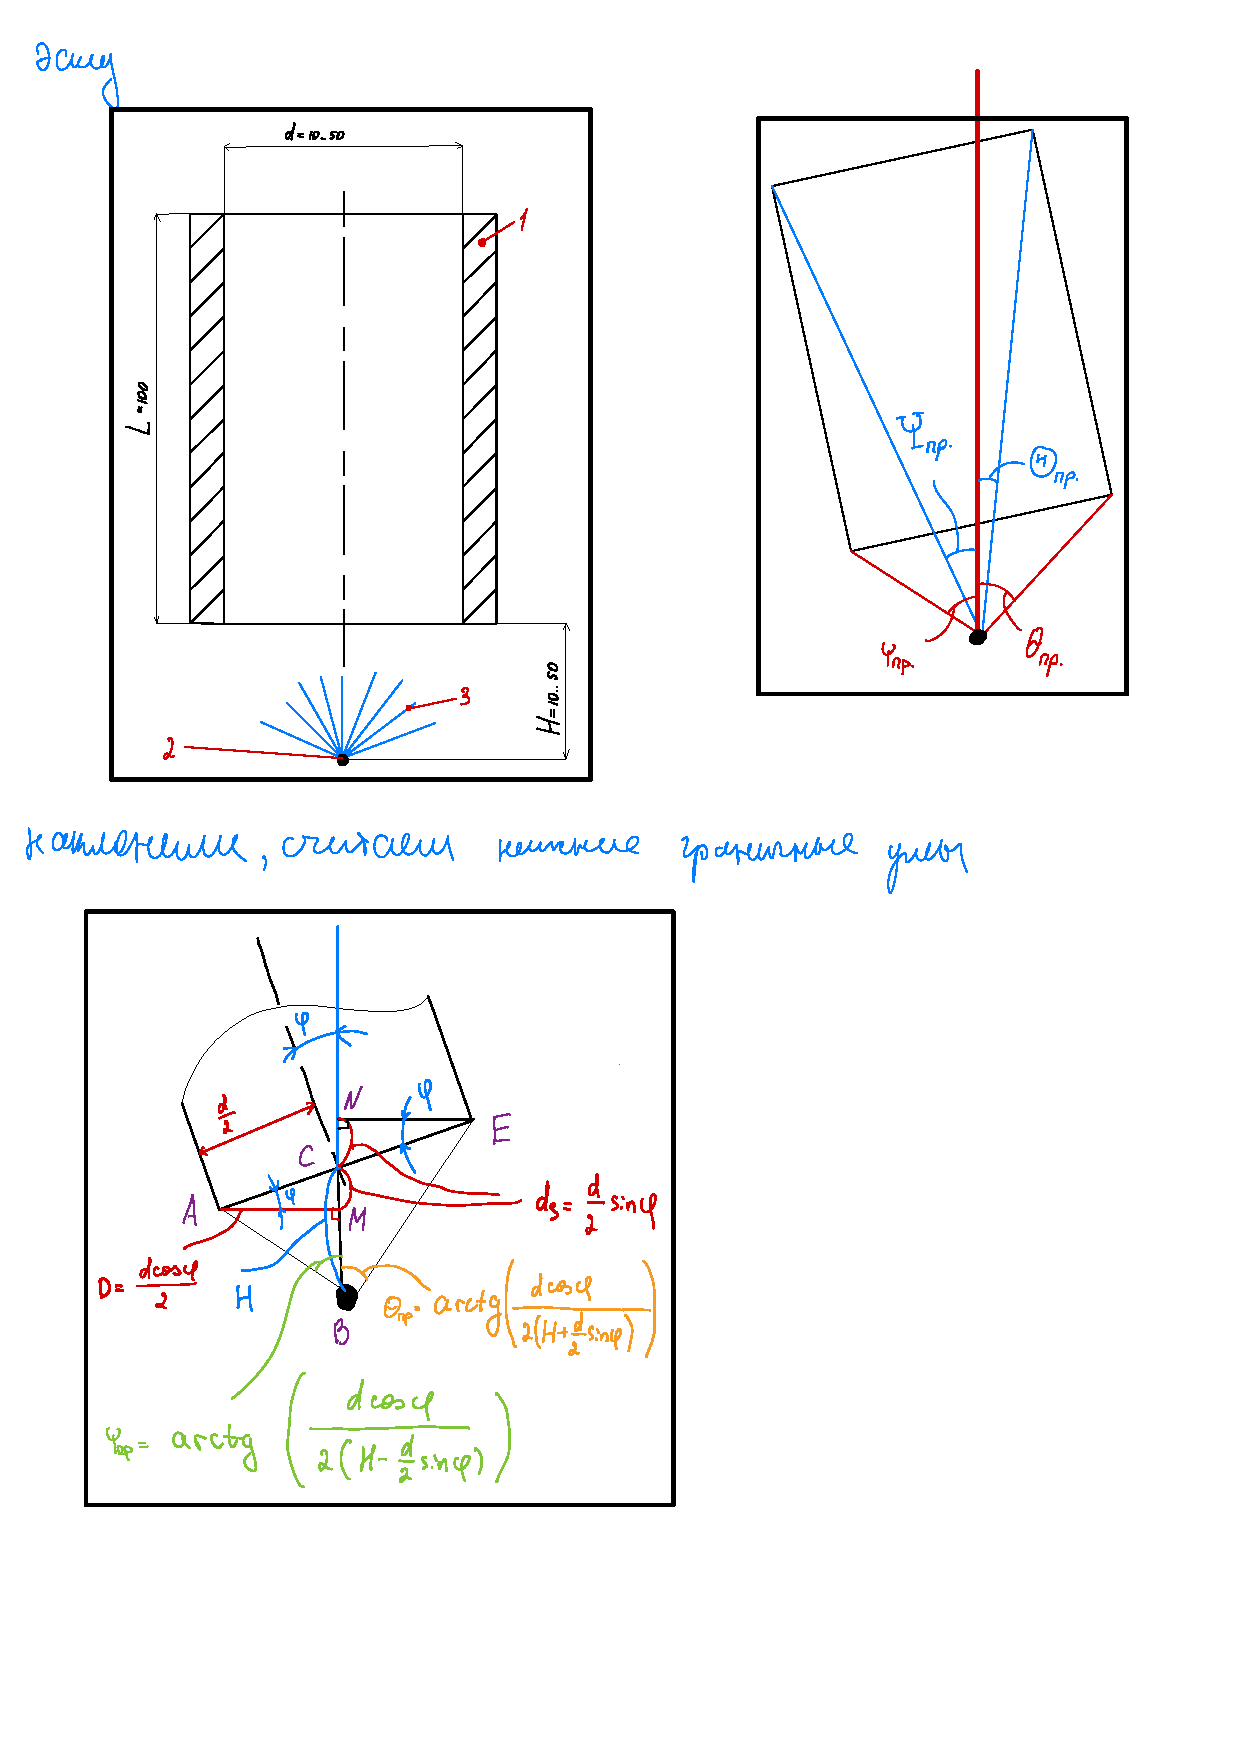
\includegraphics[trim=370 520 60 60, clip, width=0.5\linewidth]{../images/t1}
	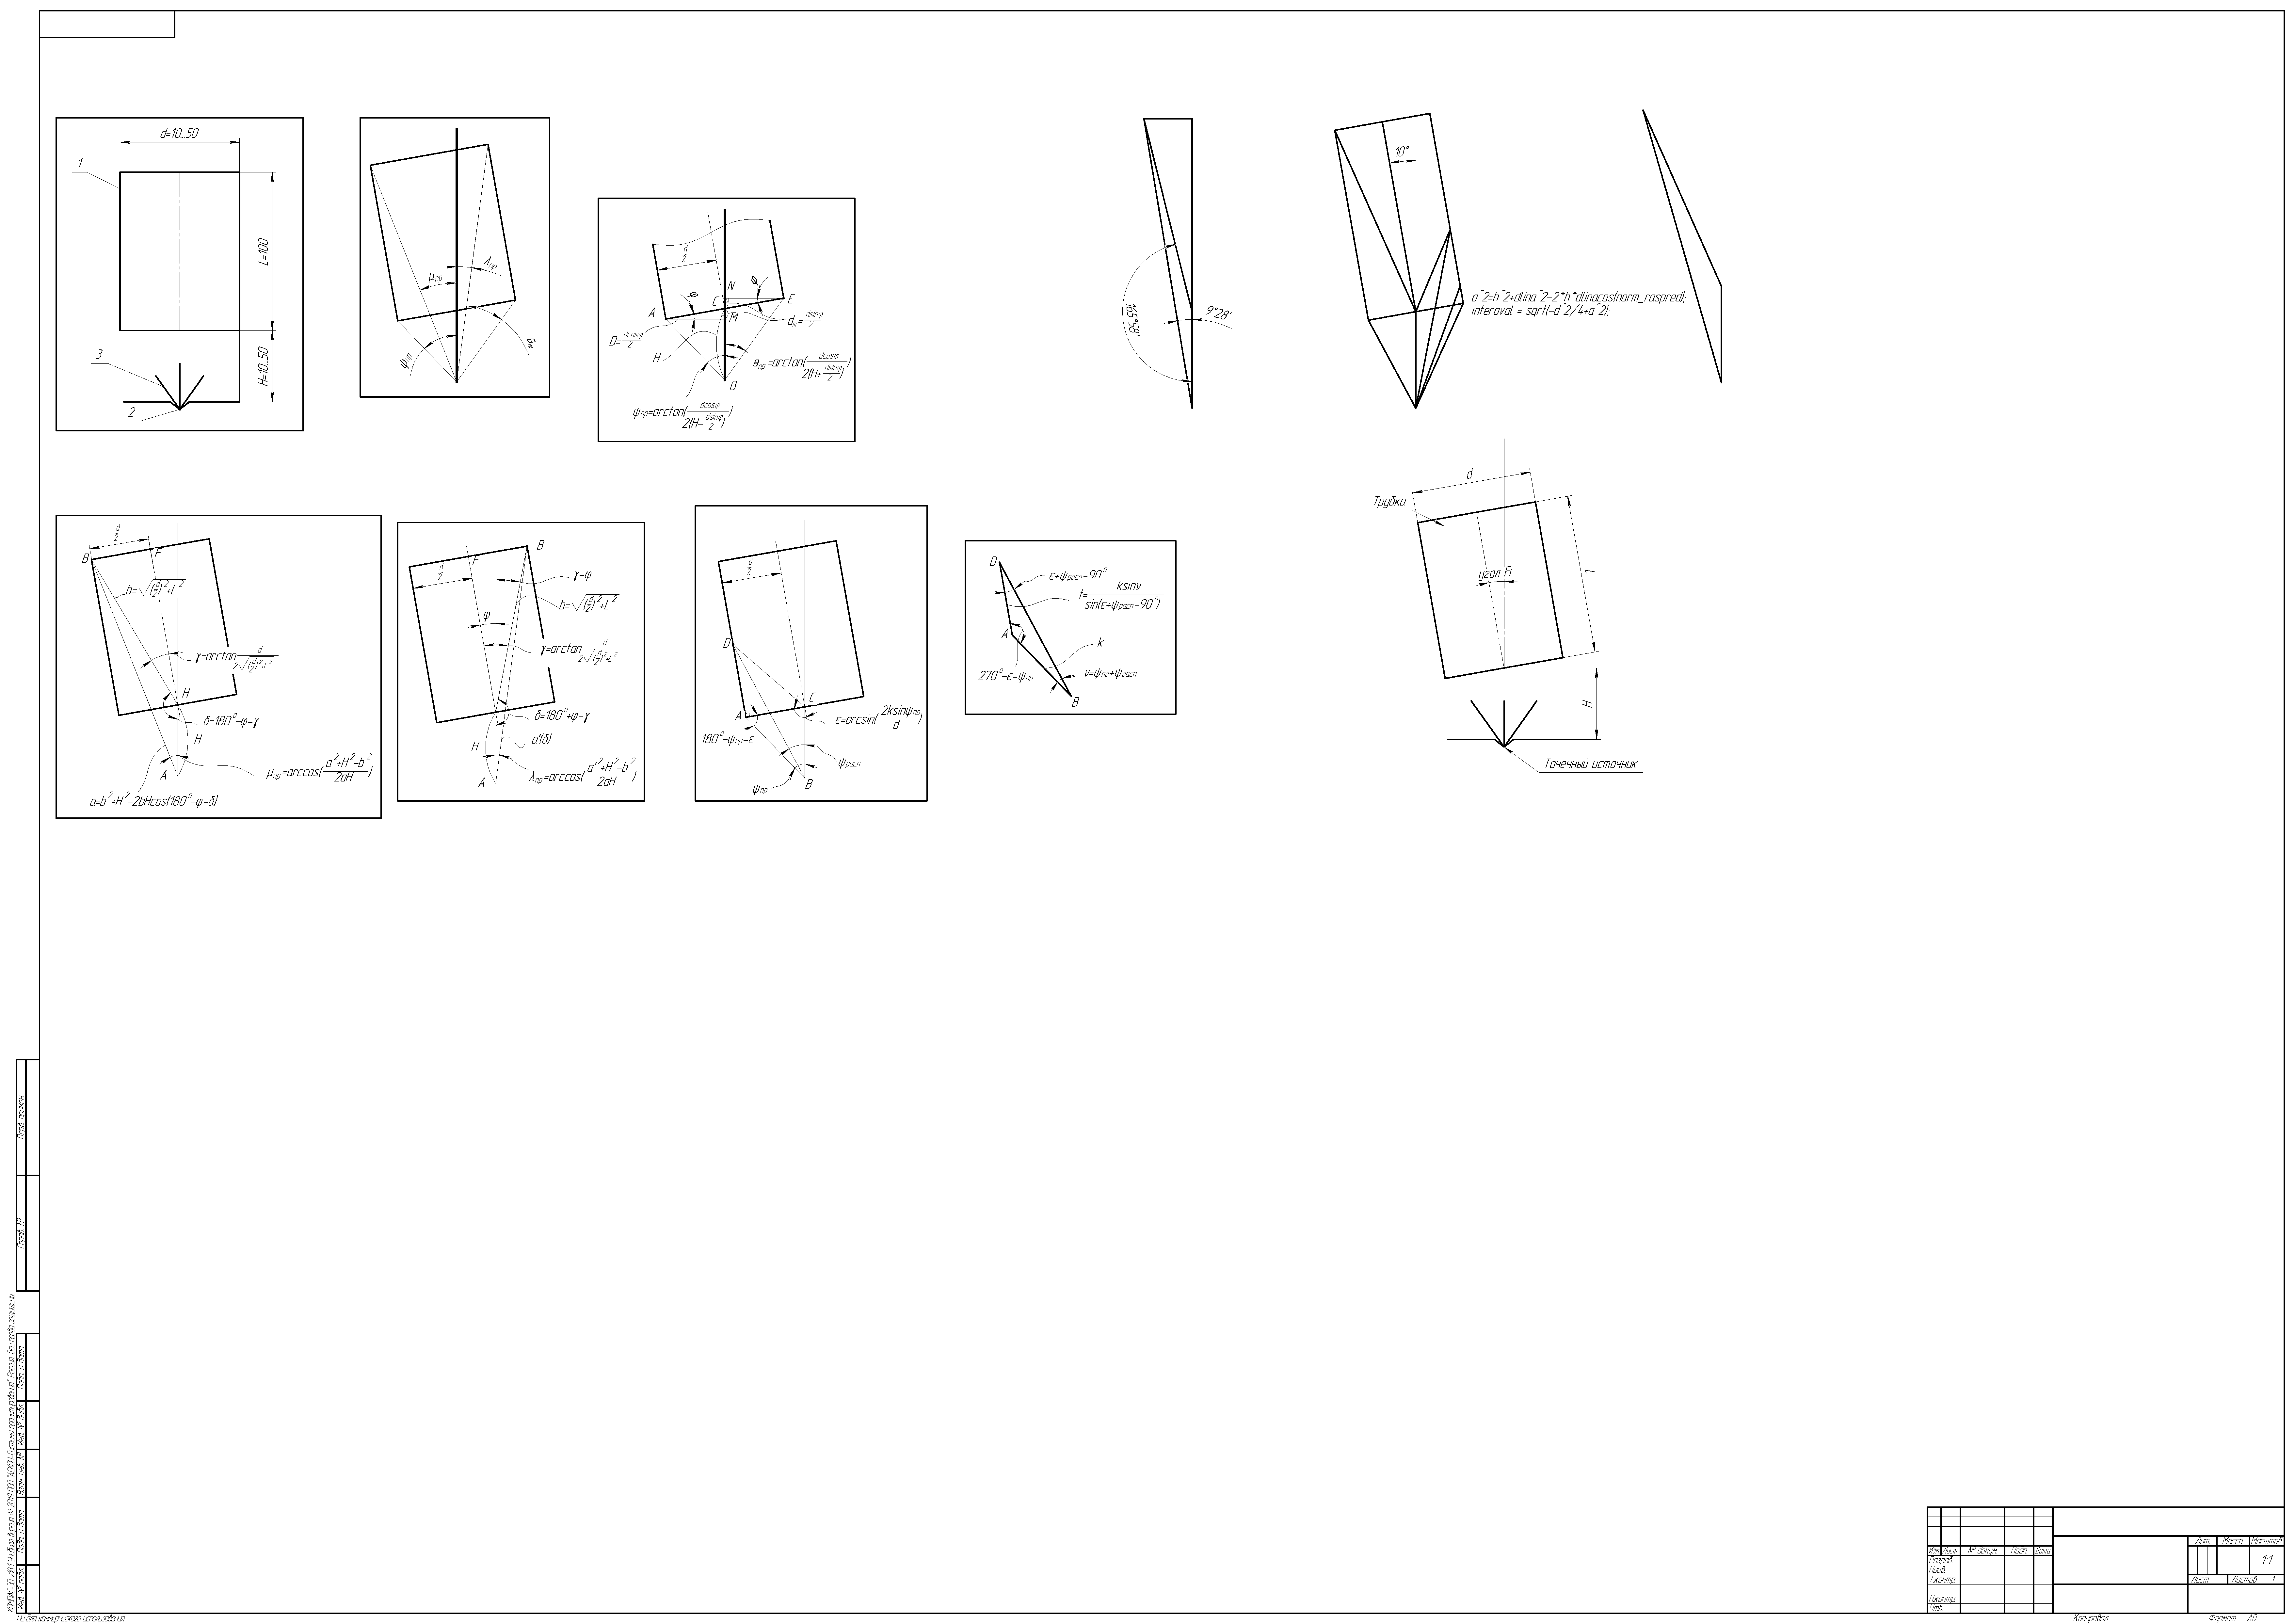
\includegraphics[trim=540 1820 2580 180, clip, width=0.5\linewidth]{../images/schemes}
	\caption{Граничные условия}
	\label{fig:border}
\end{figure}
\paragraph{Нижние граничные условия}
Рассмотрим нижнюю часть трубки для нахождения углов \lu и \ru (см. \refris{fig:niz}). В треугольнике \textit{ACB}:
\begin{equation}\label{eq:ld}
	\ld = \arctg \left(\frac{\mathit{AM}}{\mathit{BM}}\right)=\arctg \left(\frac{\frac{d\cos \phi}{2}}{H-\frac{d}{2}\sin\phi}\right)=\arctg \left(\frac{d}{\left(2\left(H-\frac{d}{2}\sin\phi\right)\right)}\right)
\end{equation}

\begin{figure}
	\centering
	%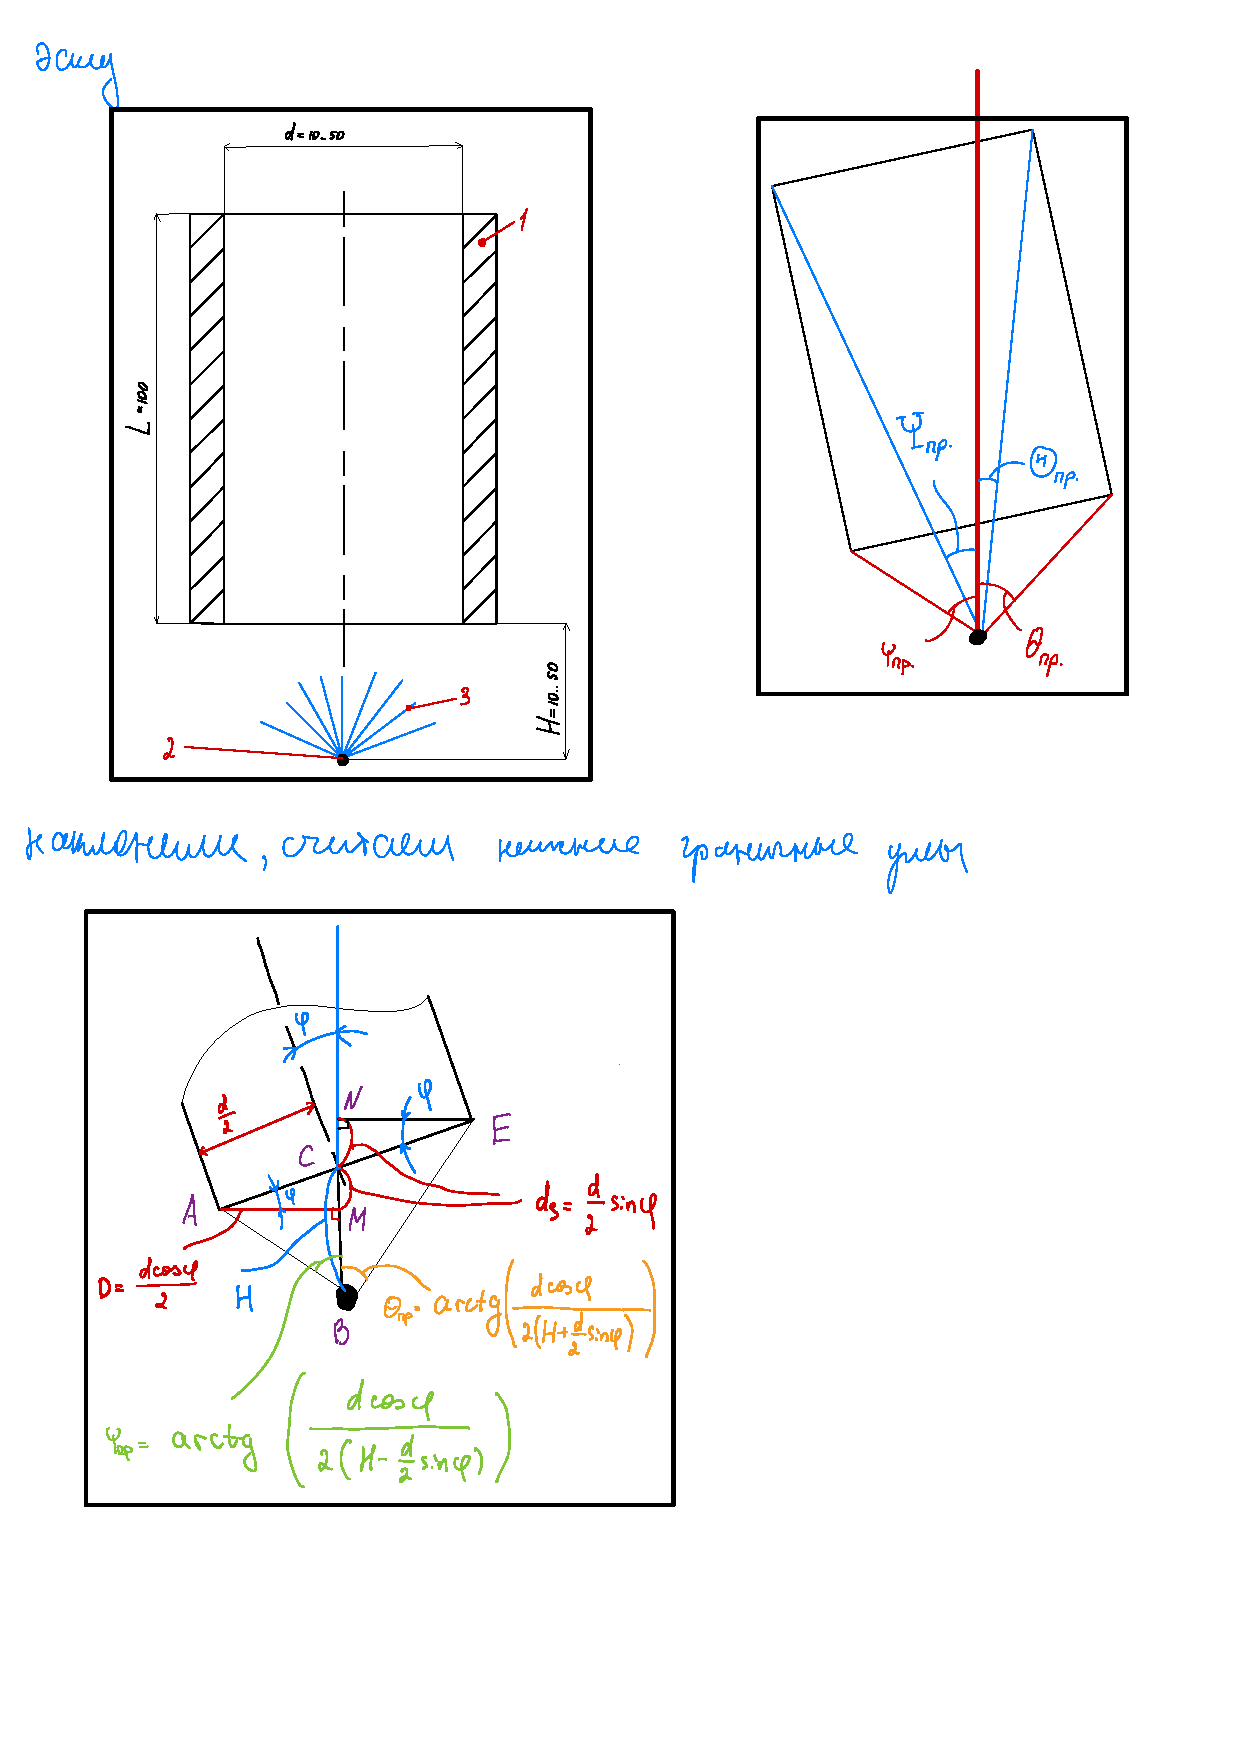
\includegraphics[trim=45 129 280 450, clip, width=0.7\linewidth]{../images/t1}
	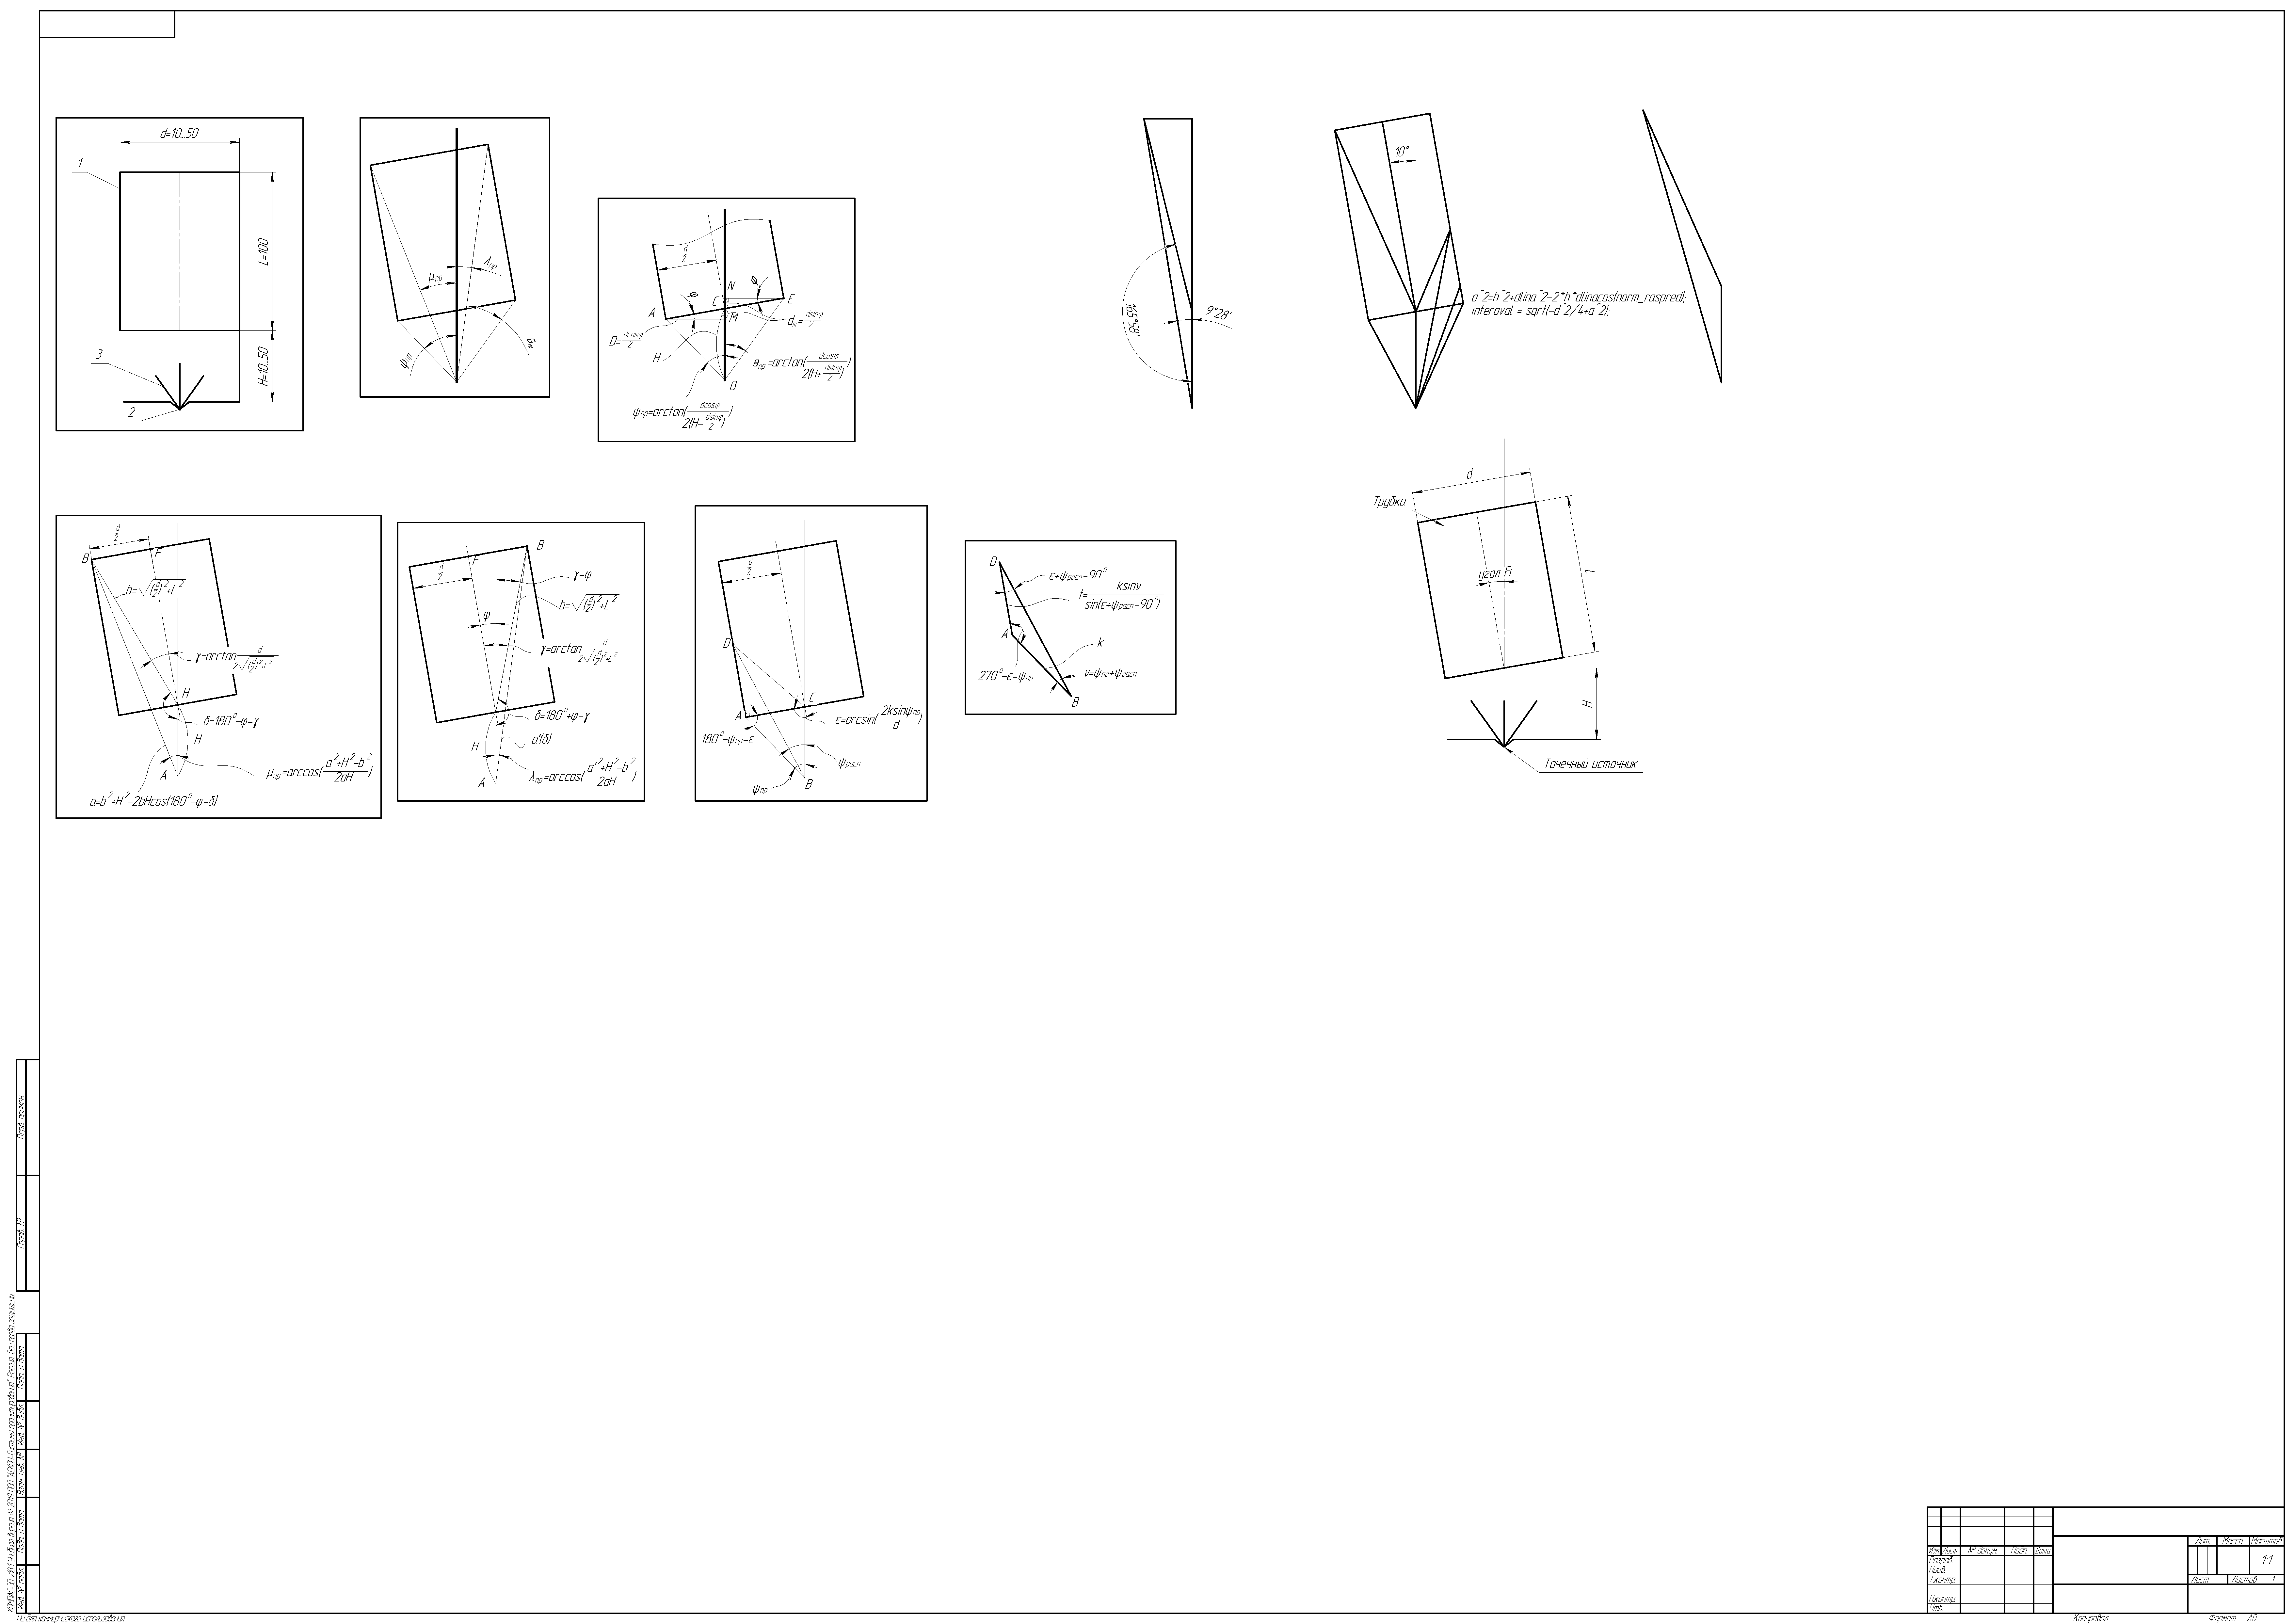
\includegraphics[trim=890 1750 2120 320, clip, width=0.7\linewidth]{../images/schemes}
	\caption{Нижние граничные условия}
	\label{fig:niz}
\end{figure}

Похожим образом найдём правое граничное условие из треугольника \textit{BNE}:
\begin{equation}
	\rd = \arctg \left(\frac{\mathit{NE}}{\mathit{BN}}\right)=\arctg \left(\frac{\frac{d\cos \phi}{2}}{H+\frac{d}{2}\sin\phi}\right)=\arctg \left(\frac{d}{\left(2\left(H+\frac{d}{2}\sin\phi\right)\right)}\right)
\end{equation}
\paragraph{Верхние граничные условия}
Рассмотрим верхнюю часть трубки (см. \refris{fig:verh}). Найдём левую границу (\refris{fig:verh_left}):
\begin{enumerate}
	\item Угол $\gamma$ из треугольника \textit{BHF}:
	\begin{equation}
		\gamma = \arctg \left(\frac{\mathit{BF}}{\mathit{BH}}\right) = \arctg\left(\frac{\frac{d}{2}}{b}\right)=\arctg \left(\frac{d}{2\sqrt{\left(\frac{d}{2}\right)^2+L^2}}\right)
	\end{equation}
	\item Угол \textit{AHB}:
	\begin{equation}
		\mathit{AHB} = \delta = 180\grad-\phi-\gamma
	\end{equation}
	\item В треугольнике \textit{AHB} по теореме косинусов находим сторону  $a$:
	\begin{equation}
		a = b^2 + H^2 - 2bH \cos \left(180\grad - \phi - \delta\right)
	\end{equation}
	\item По теореме косинусов треугольника \textit{AHB} находим искомый угол:
	\begin{aleq}
		b^2 &= a^2+H^2=2aH\cos\left(\lu\right)\\
		\lu &= \arccos \left(\frac{a^2+H^2-b^2}{2aH}\right)		
	\end{aleq}
\end{enumerate}
\begin{figure}[p]
	\begin{subfigure}{0.5\linewidth}
		\centering
		%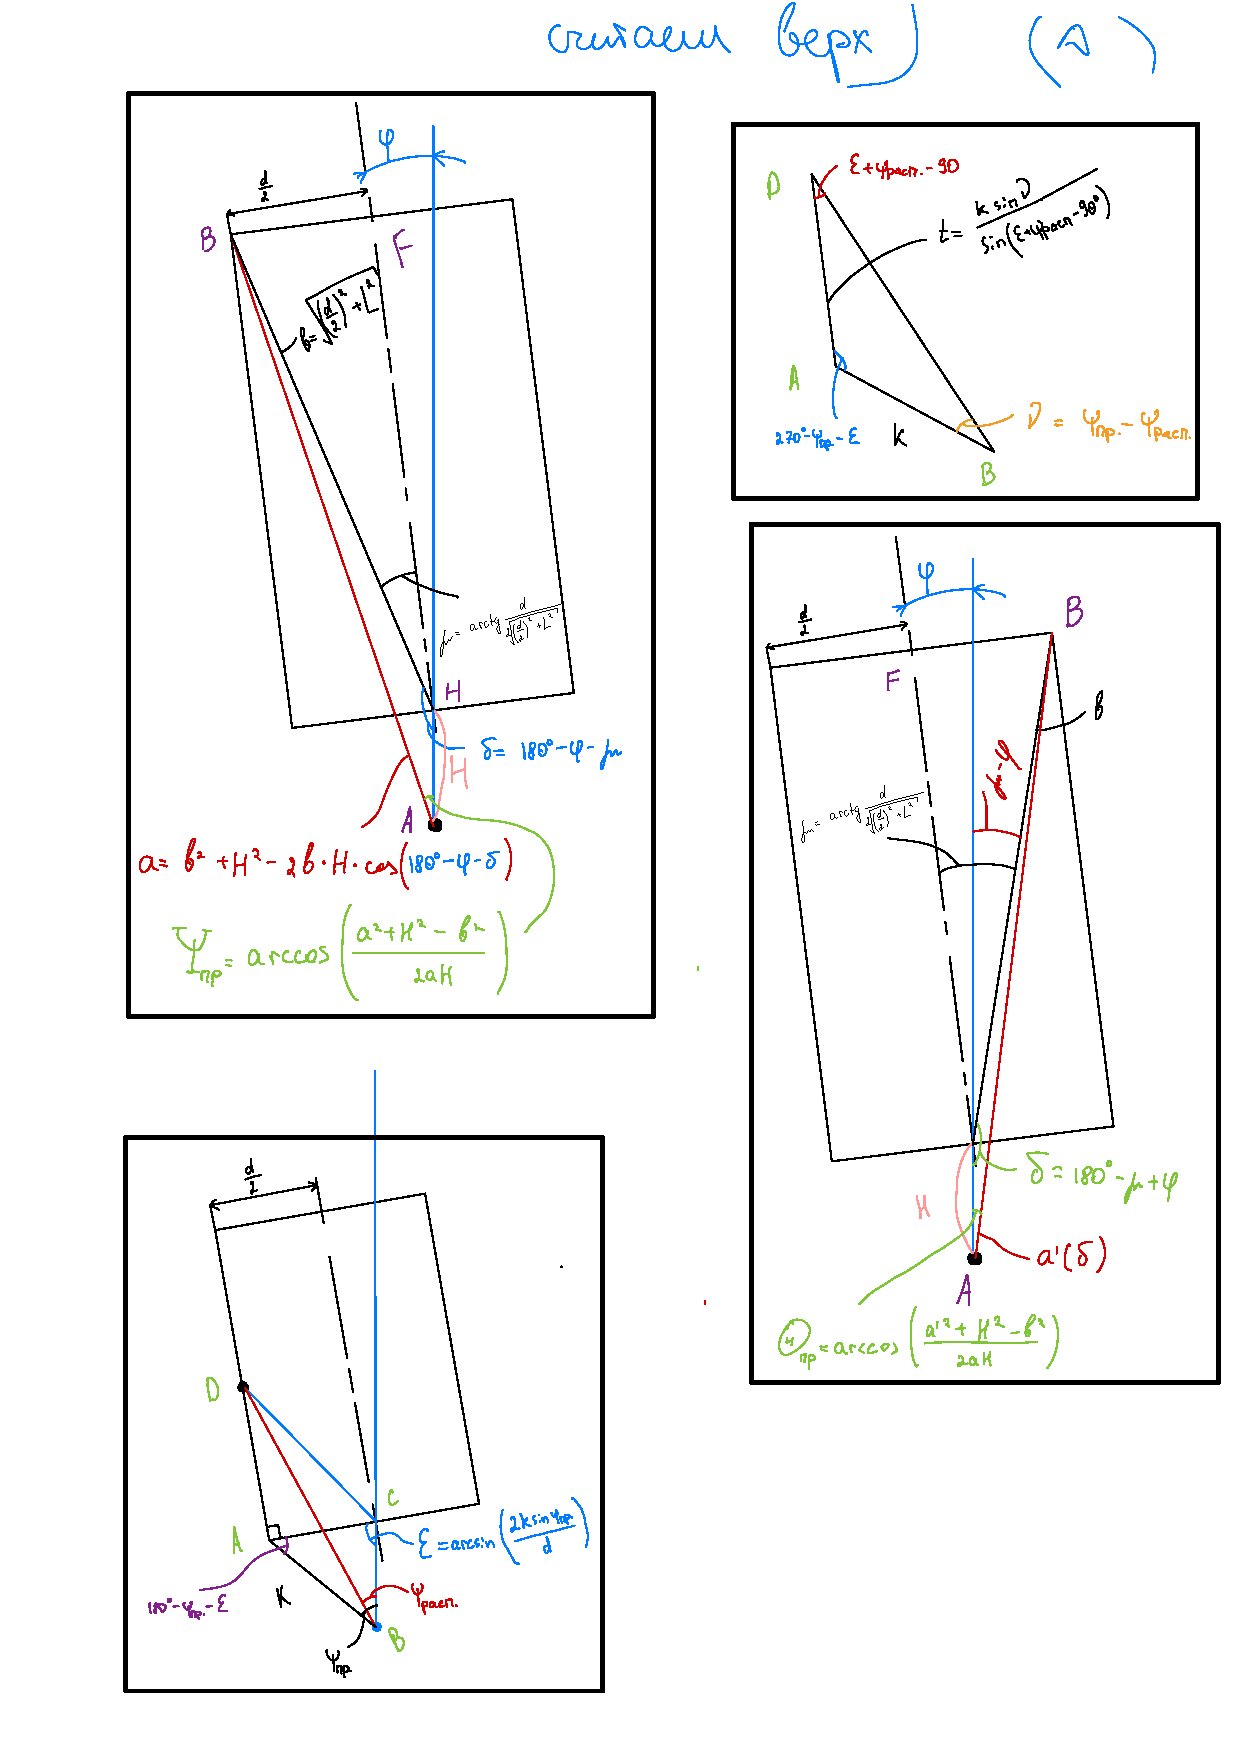
\includegraphics[trim=65 370 300 55,clip, height=1.3\linewidth]{../images/t2}
		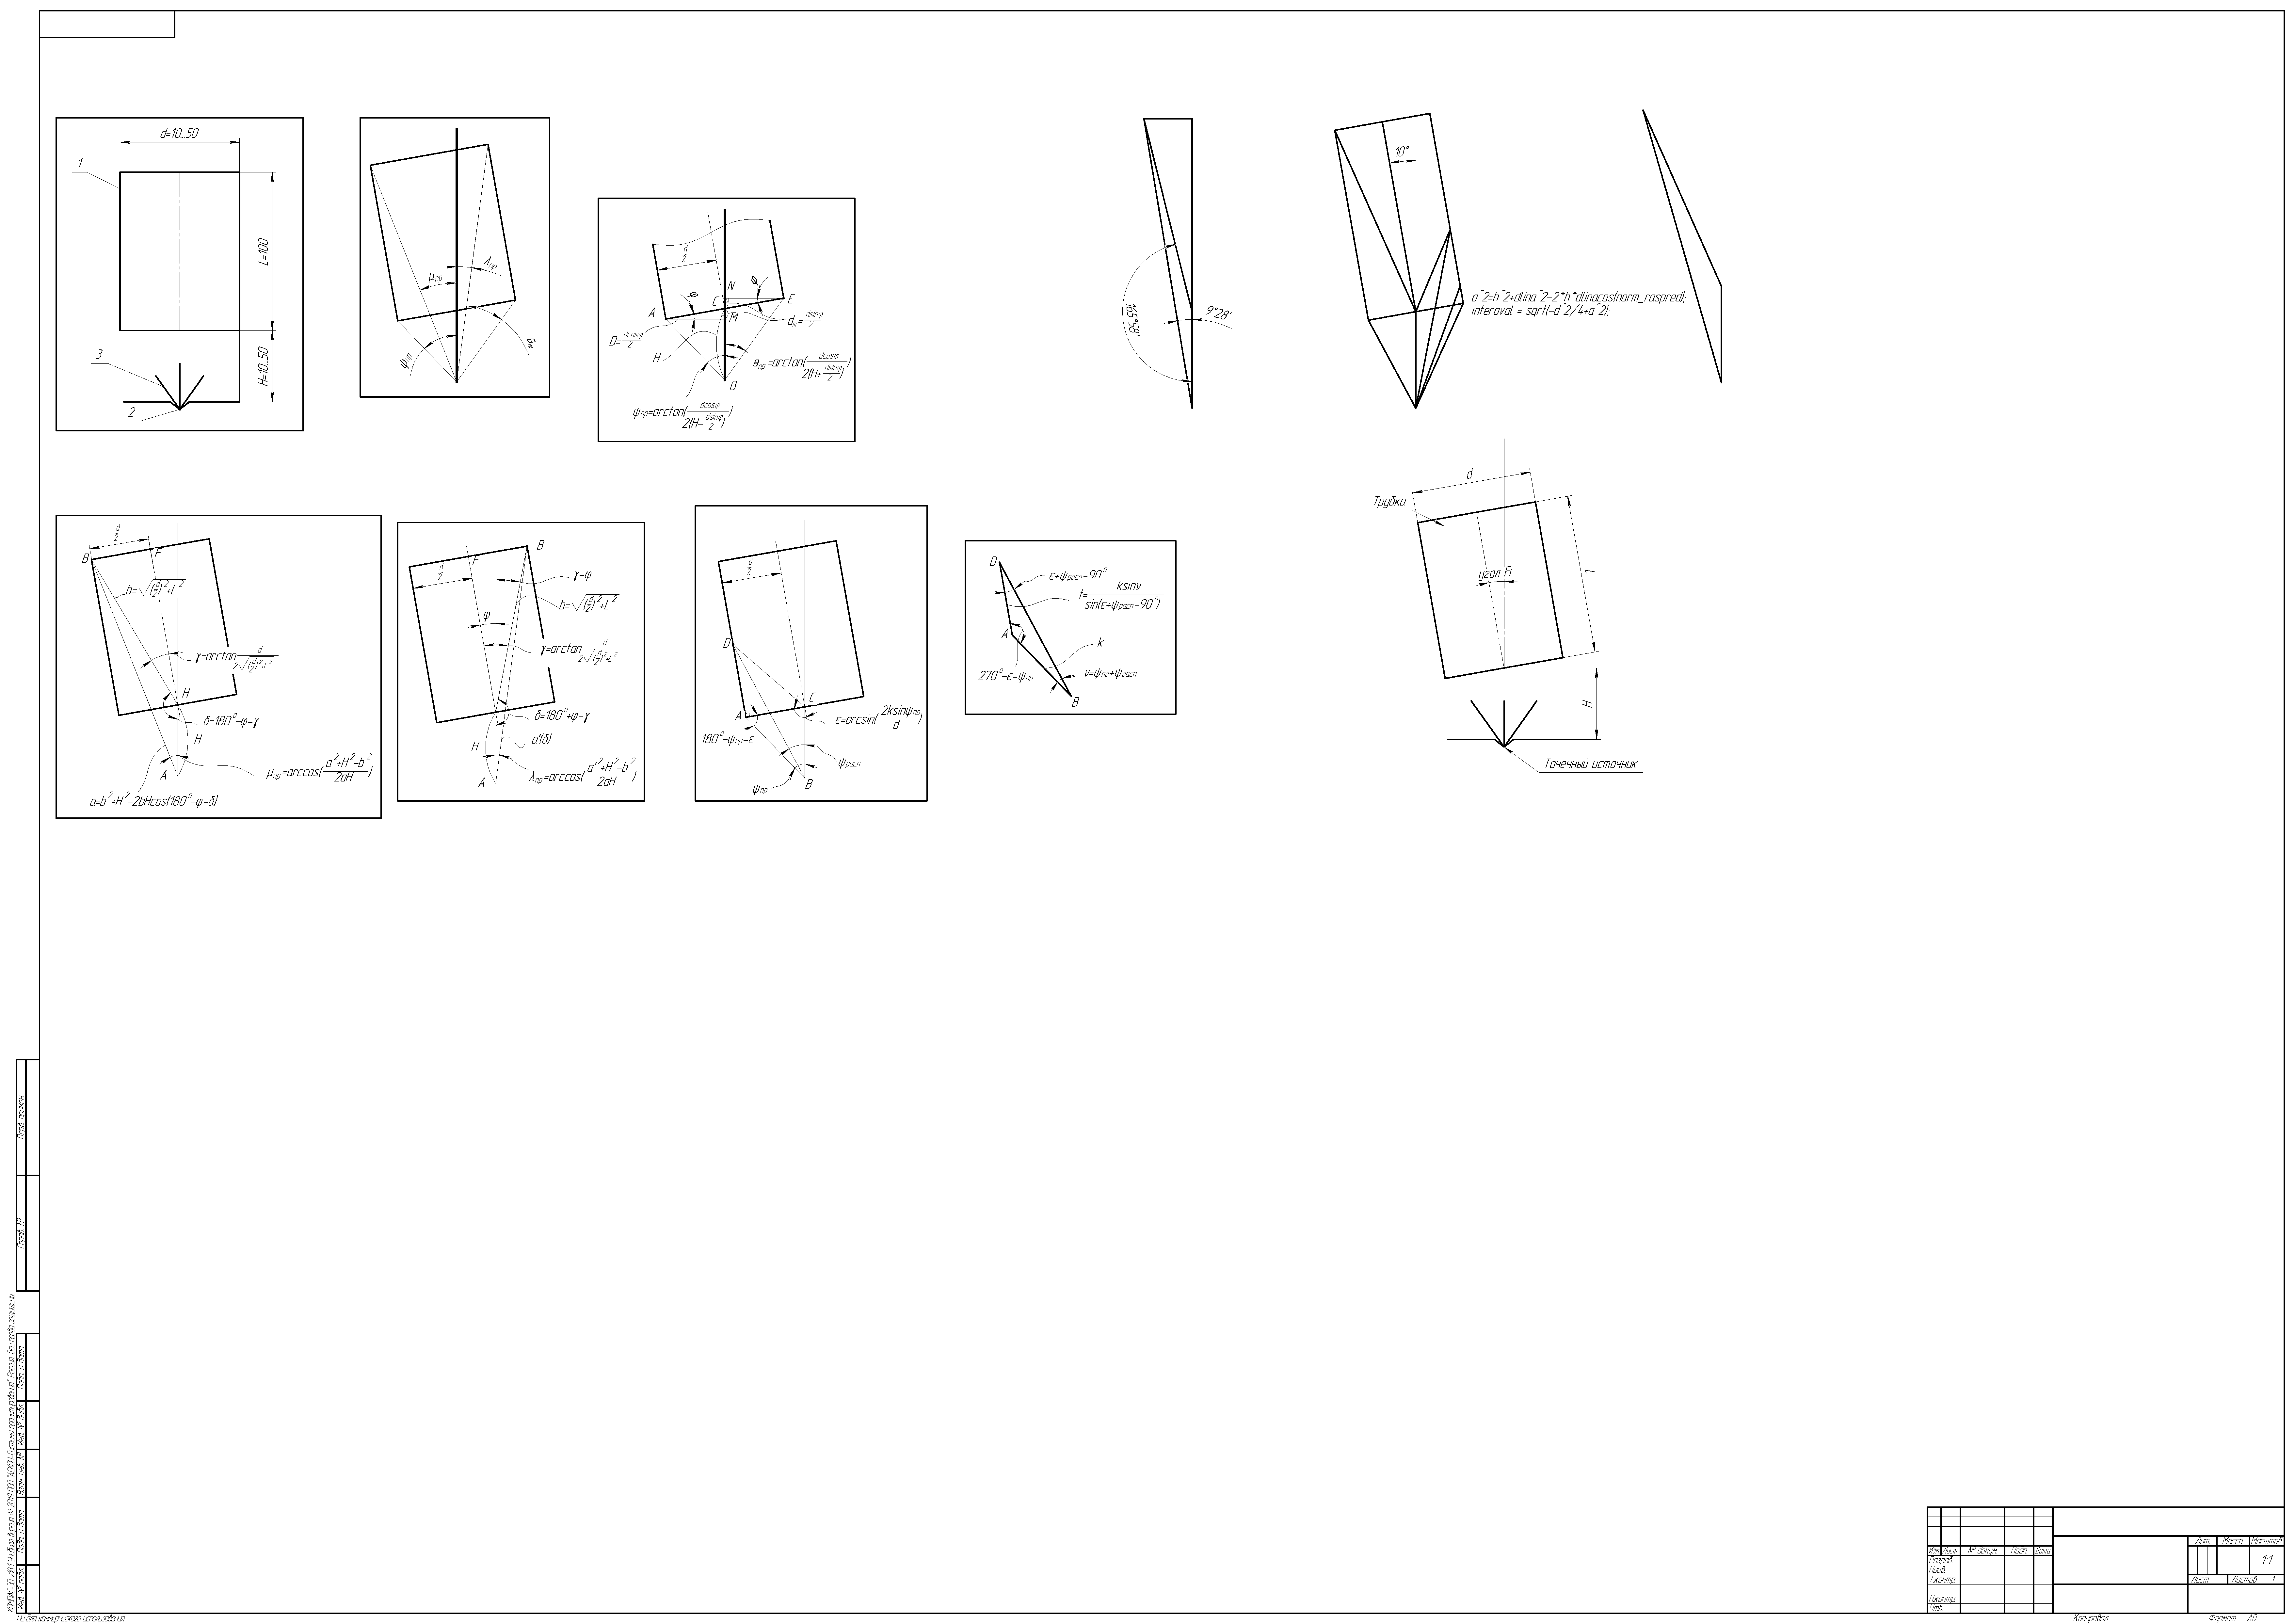
\includegraphics[trim=100 1200 2820 760, clip, height=1.1\linewidth]{../images/schemes}
		\caption{Верхнее левое граничное условие}
		\label{fig:verh_left}
	\end{subfigure}
	\begin{subfigure}{0.5\linewidth}
		\centering
		%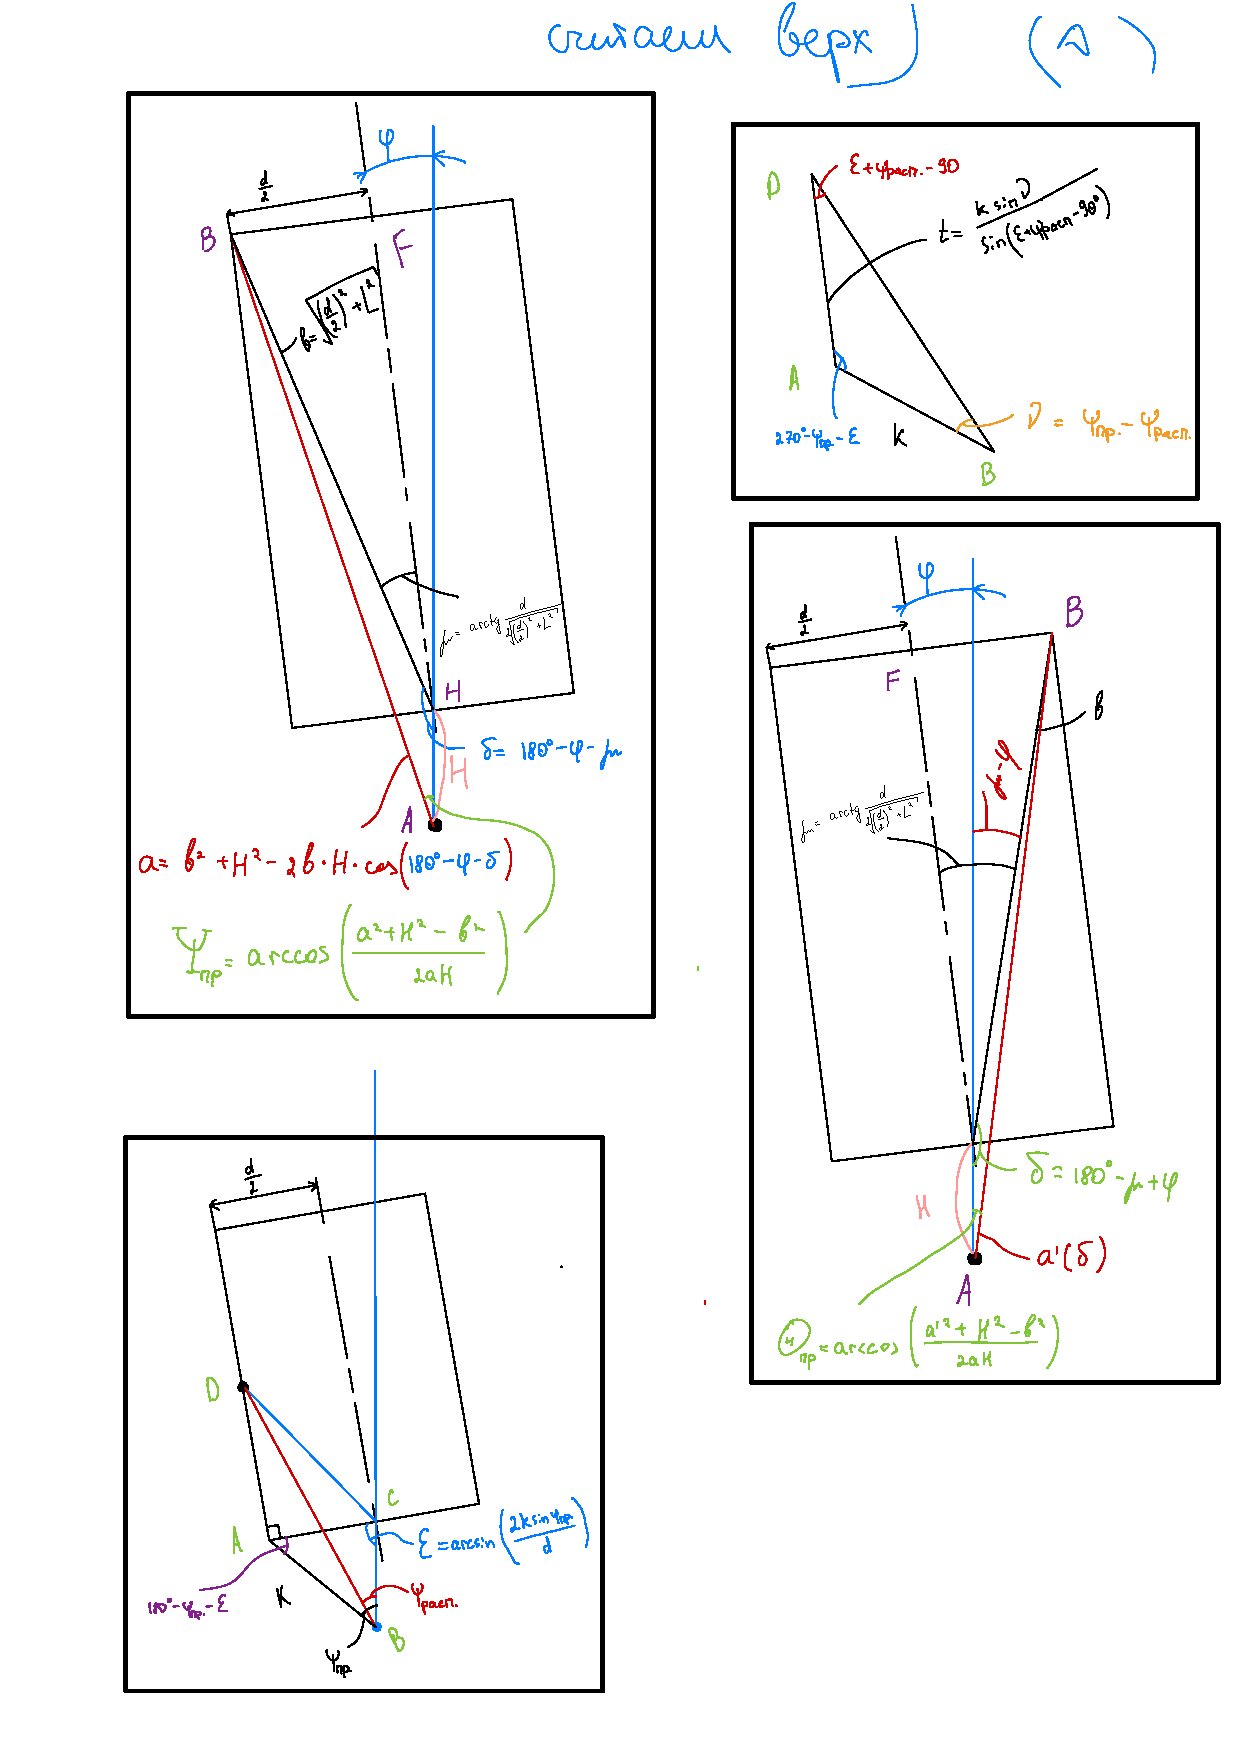
\includegraphics[trim=365 185 30 260,clip, height=1.3\linewidth]{../images/t2}
		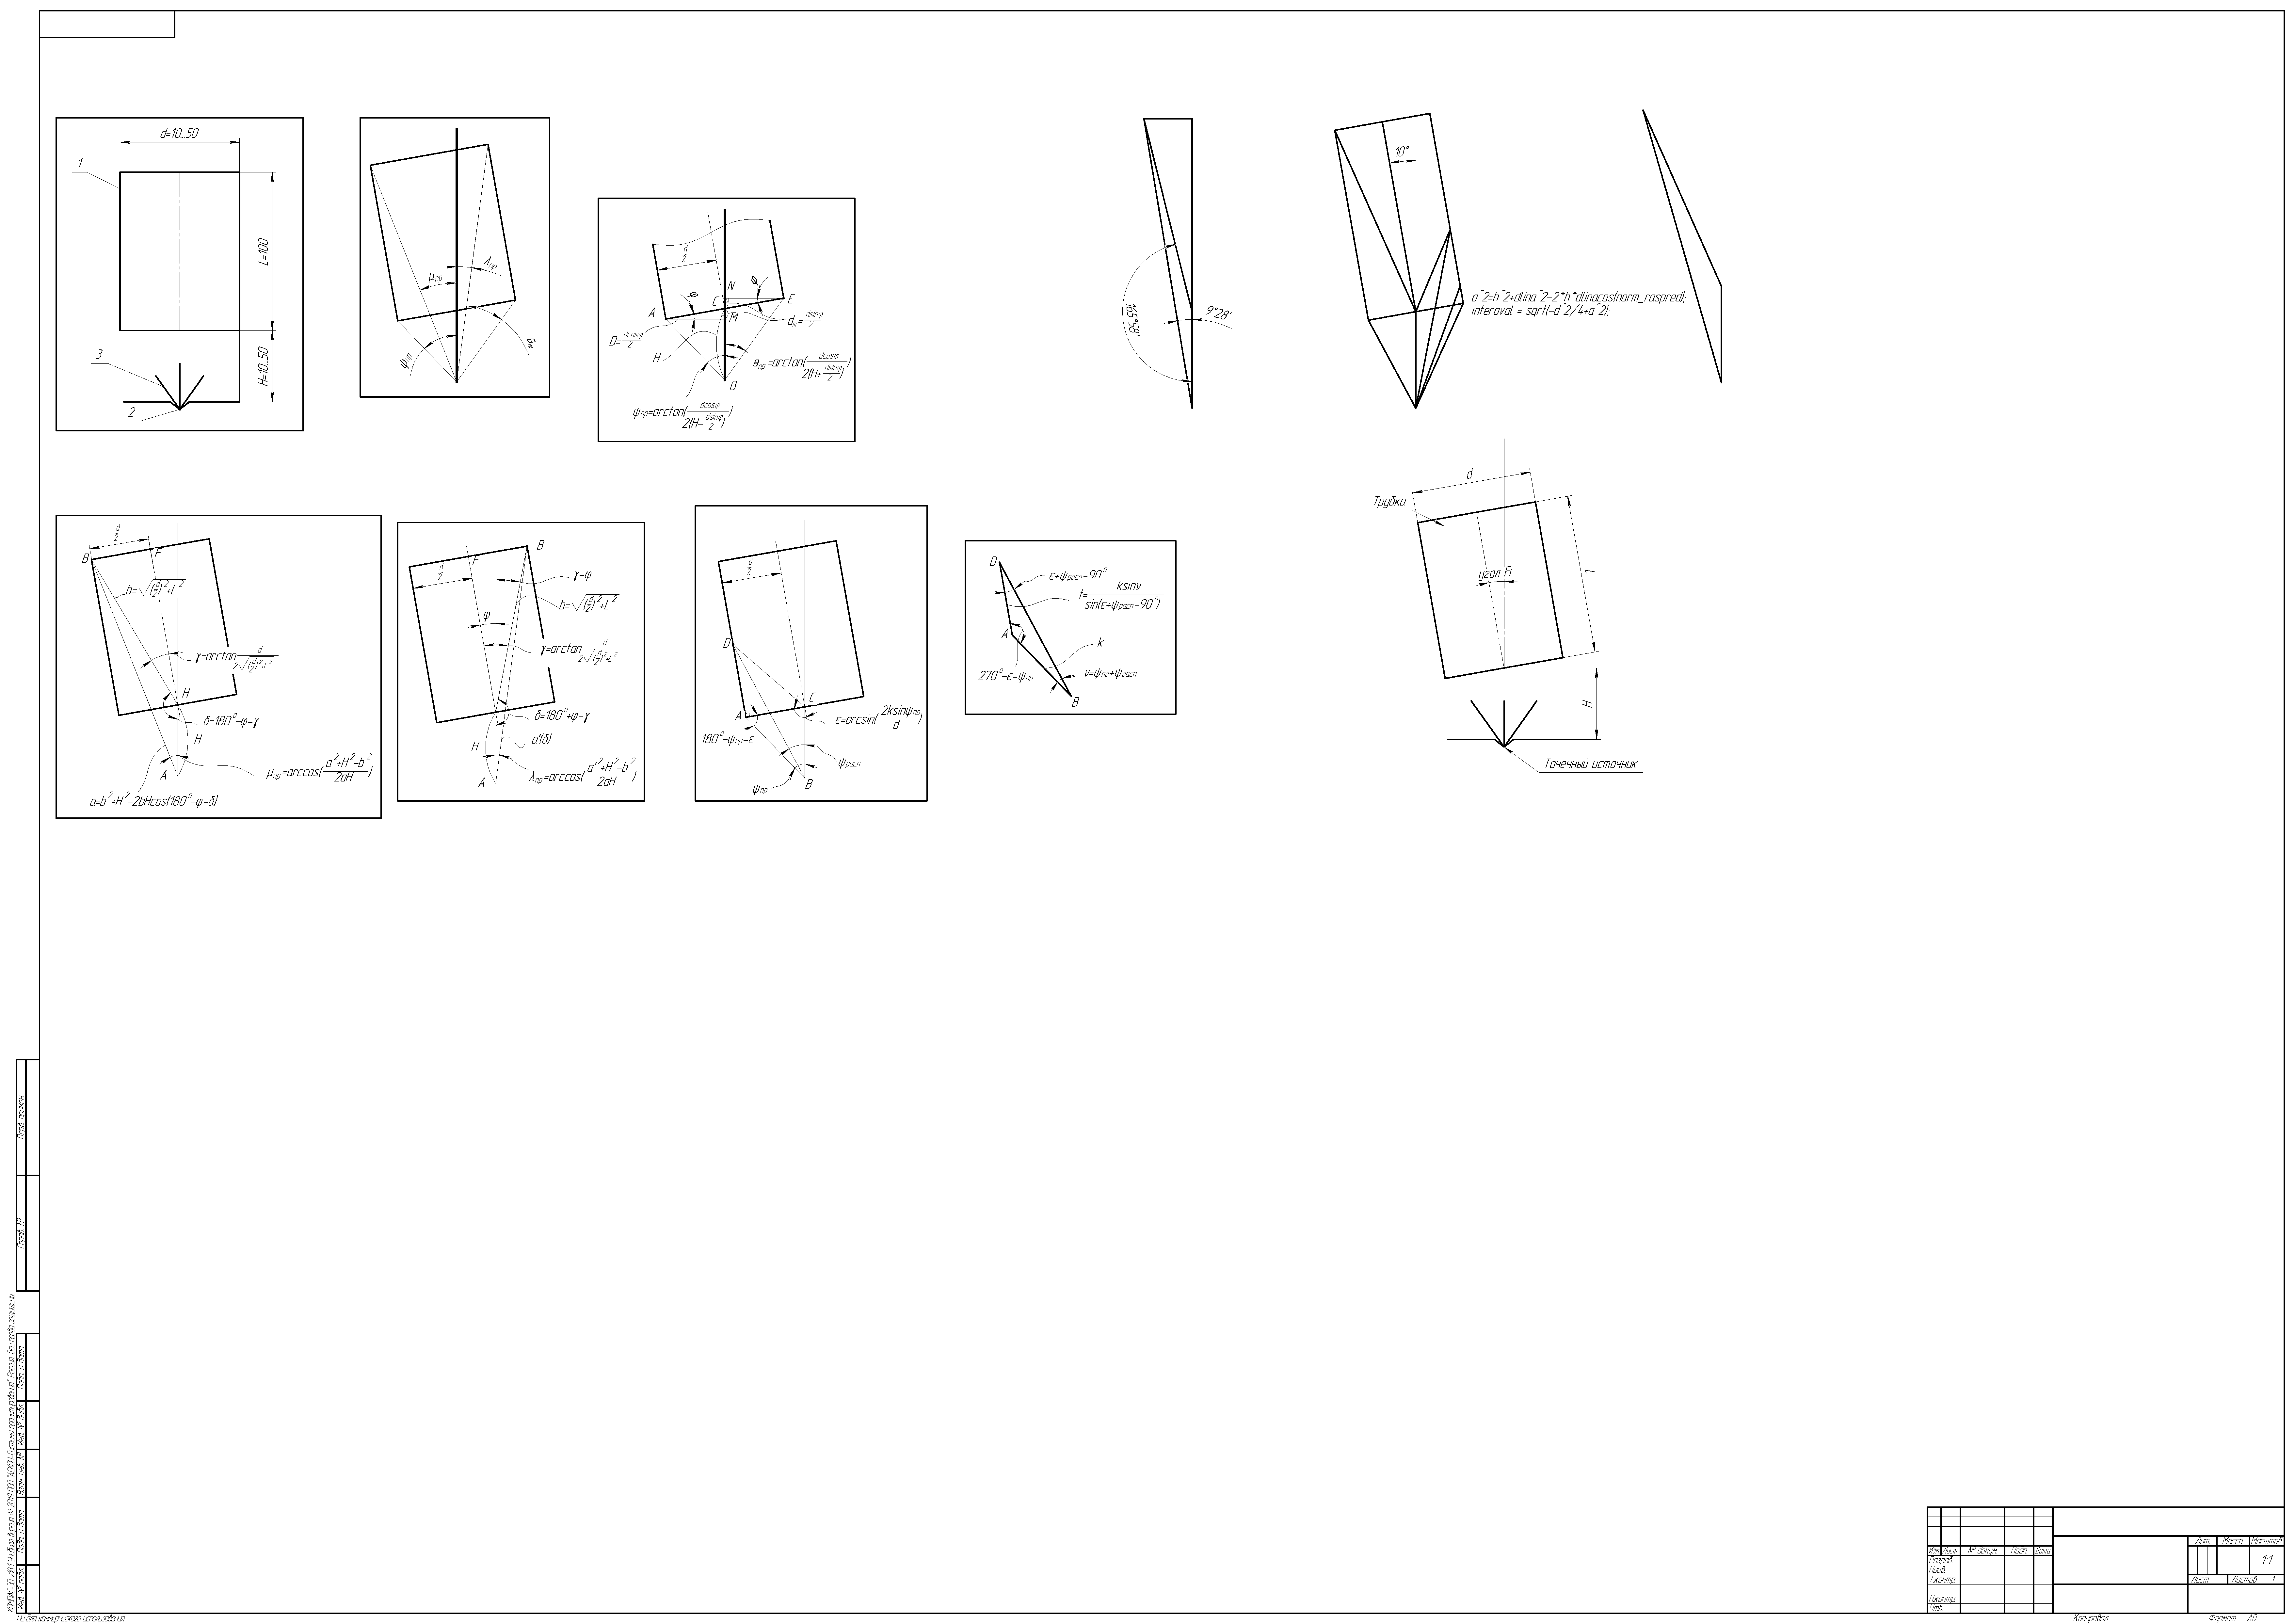
\includegraphics[trim=600 1220 2430 790, clip, height=1.1\linewidth]{../images/schemes}
		\caption{Верхнее правое граничное условие}
		\label{fig:verh_right}
	\end{subfigure}
	\caption{Верхние граничные условия}
	\label{fig:verh}
\end{figure}
Правое граничное условие может быть найдено по аналогии (см. \refris{fig:verh_right}):
\begin{aleq}
	b^2 &= a^2+H^2=2aH\cos\left(\ru\right)\\
	\ru &= \arccos \left(\frac{a^2+H^2-b^2}{2aH}\right)		
\end{aleq}
\paragraph{Нахождение интервала попадания}
Как уже было сказано в \refpar{par:resume}, программа вычисляет координату попадания молекулы на сторону. На \refris{fig:monte-carlo} изображены расчётные схемы для координат молекул. 

\begin{enumerate}
	\item В треугольнике \textit{BCD} (\refris{fig:calculate}) известны стороны \textit{AB} (можно найти из \refris{fig:niz}), \xspace $\mathit{BD}=\frac{d}{2}$ и граничный угол \ld (см. уравнение \eqref{eq:ld}).  Находим углы \xspace $\epsilon$ и \xspace $\angle$\textit{CAB}:
	\begin{aleq}
		\epsilon &= \arcsin \left(\frac{2k\sin\ld}{d}\right)\\
		\angle\mathit{CAB} &= 180\grad - \ld - \epsilon
	\end{aleq}
	\item В треугольнике \textit{DAB} (см. \refris{fig:BAD}) находим углы \xspace $\angle \mathit{ADB}$ \xspace и \xspace $\angle \mathit{ADB}$:
	\begin{aleq}
		\angle \mathit{ABD} &= \ld - \fr\\
		\angle \mathit{DAB} &= 90\grad + \angle \mathit{CAB} = 90\grad + 180\grad - \ld - \epsilon = 270\grad-\ld-\epsilon\\
		\angle \mathit{ADB} &= 180\grad - \angle \mathit{DAB} - \angle \mathit{ABD} =\\
		&= 180\grad - 270\grad+\ld +\epsilon - \ld+\fr = \epsilon + \fr -90\grad
	\end{aleq}
	\item По теореме синусов треугольника \textit{ADB} находим искомую сторону (координату распыления):
	\begin{equation}
		\mathit{AD} = \frac{\mathit{AB}\sin \left(\angle \mathit{ABD}\right)}{\sin\left(\angle\mathit{ADB}\right)}
	\end{equation}
\end{enumerate}
\begin{figure}[p]
	\begin{subfigure}{0.5\linewidth}
		\centering
		%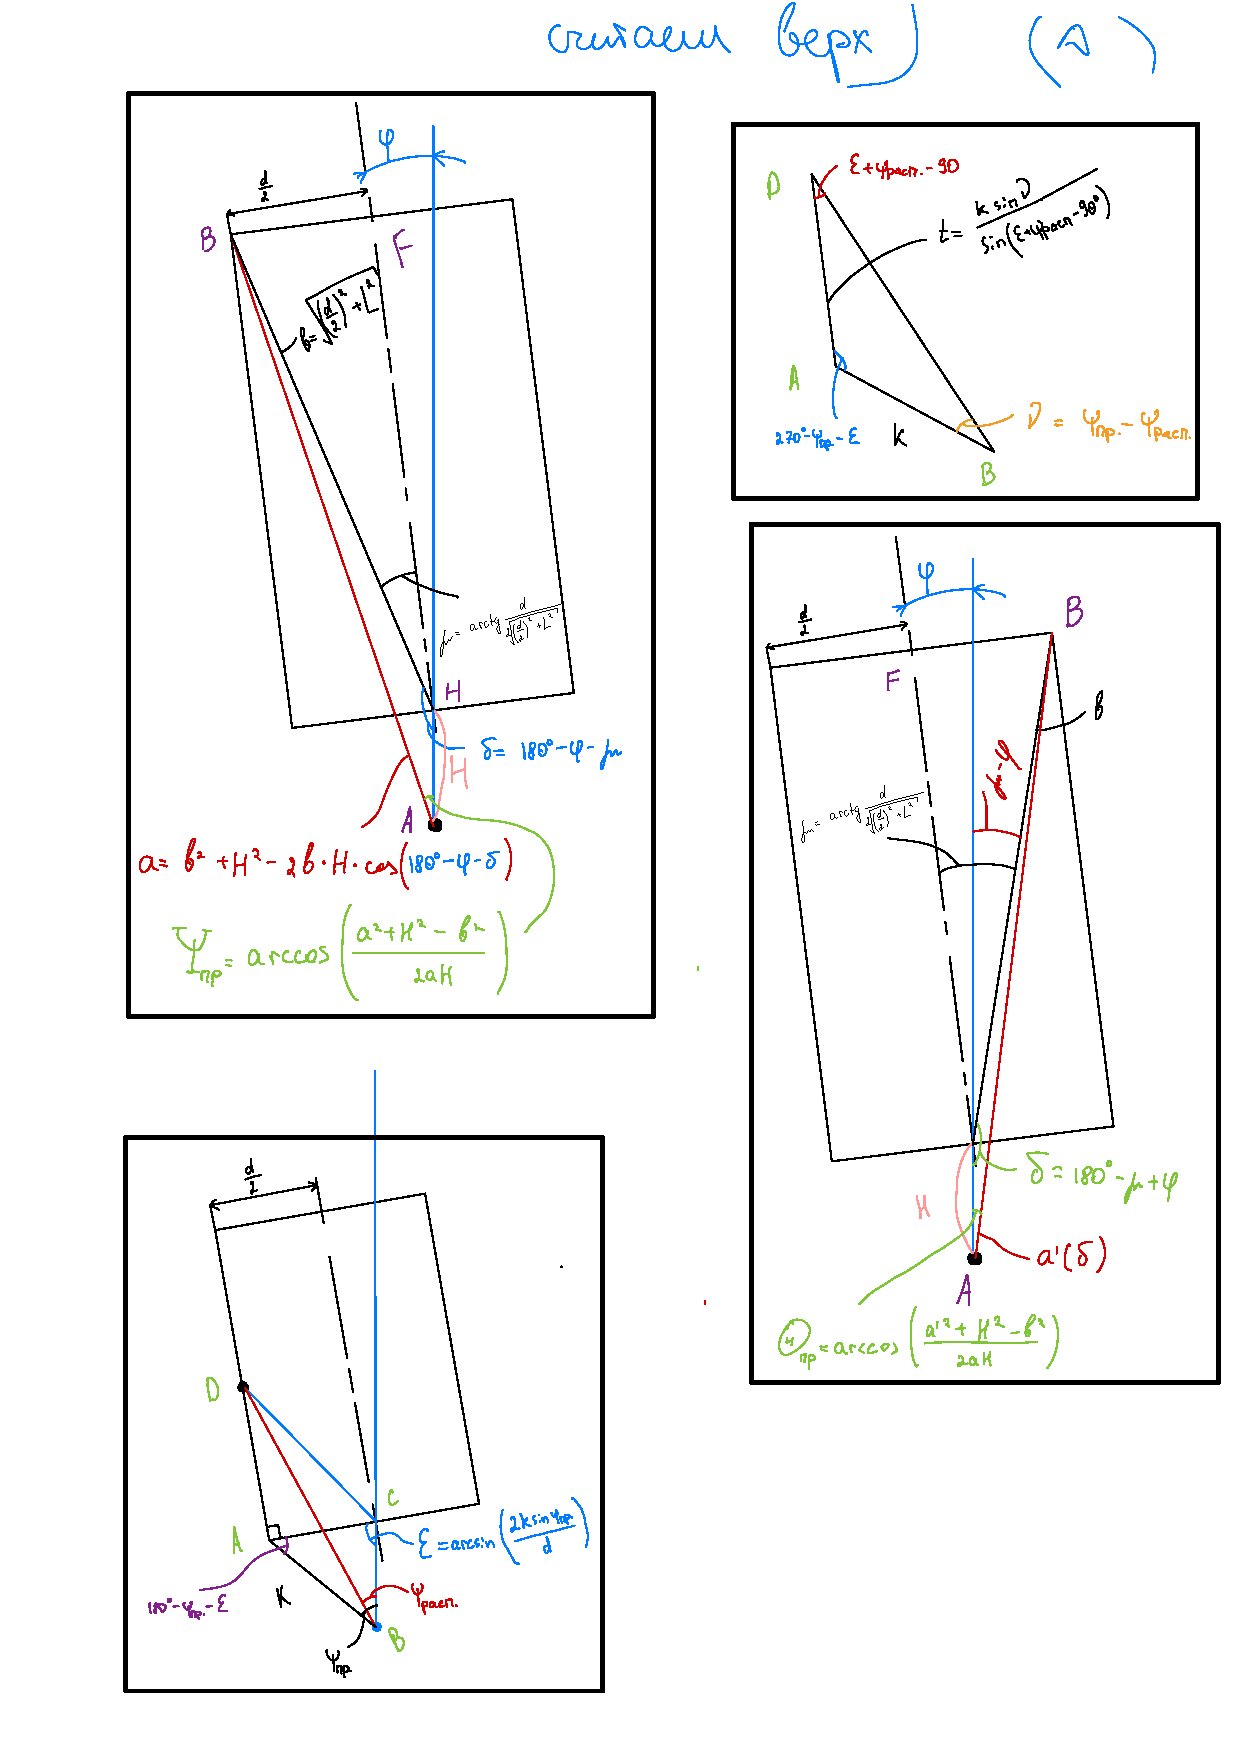
\includegraphics[trim=70 45 310 550, clip,height=0.8\linewidth]{../images/t2}
		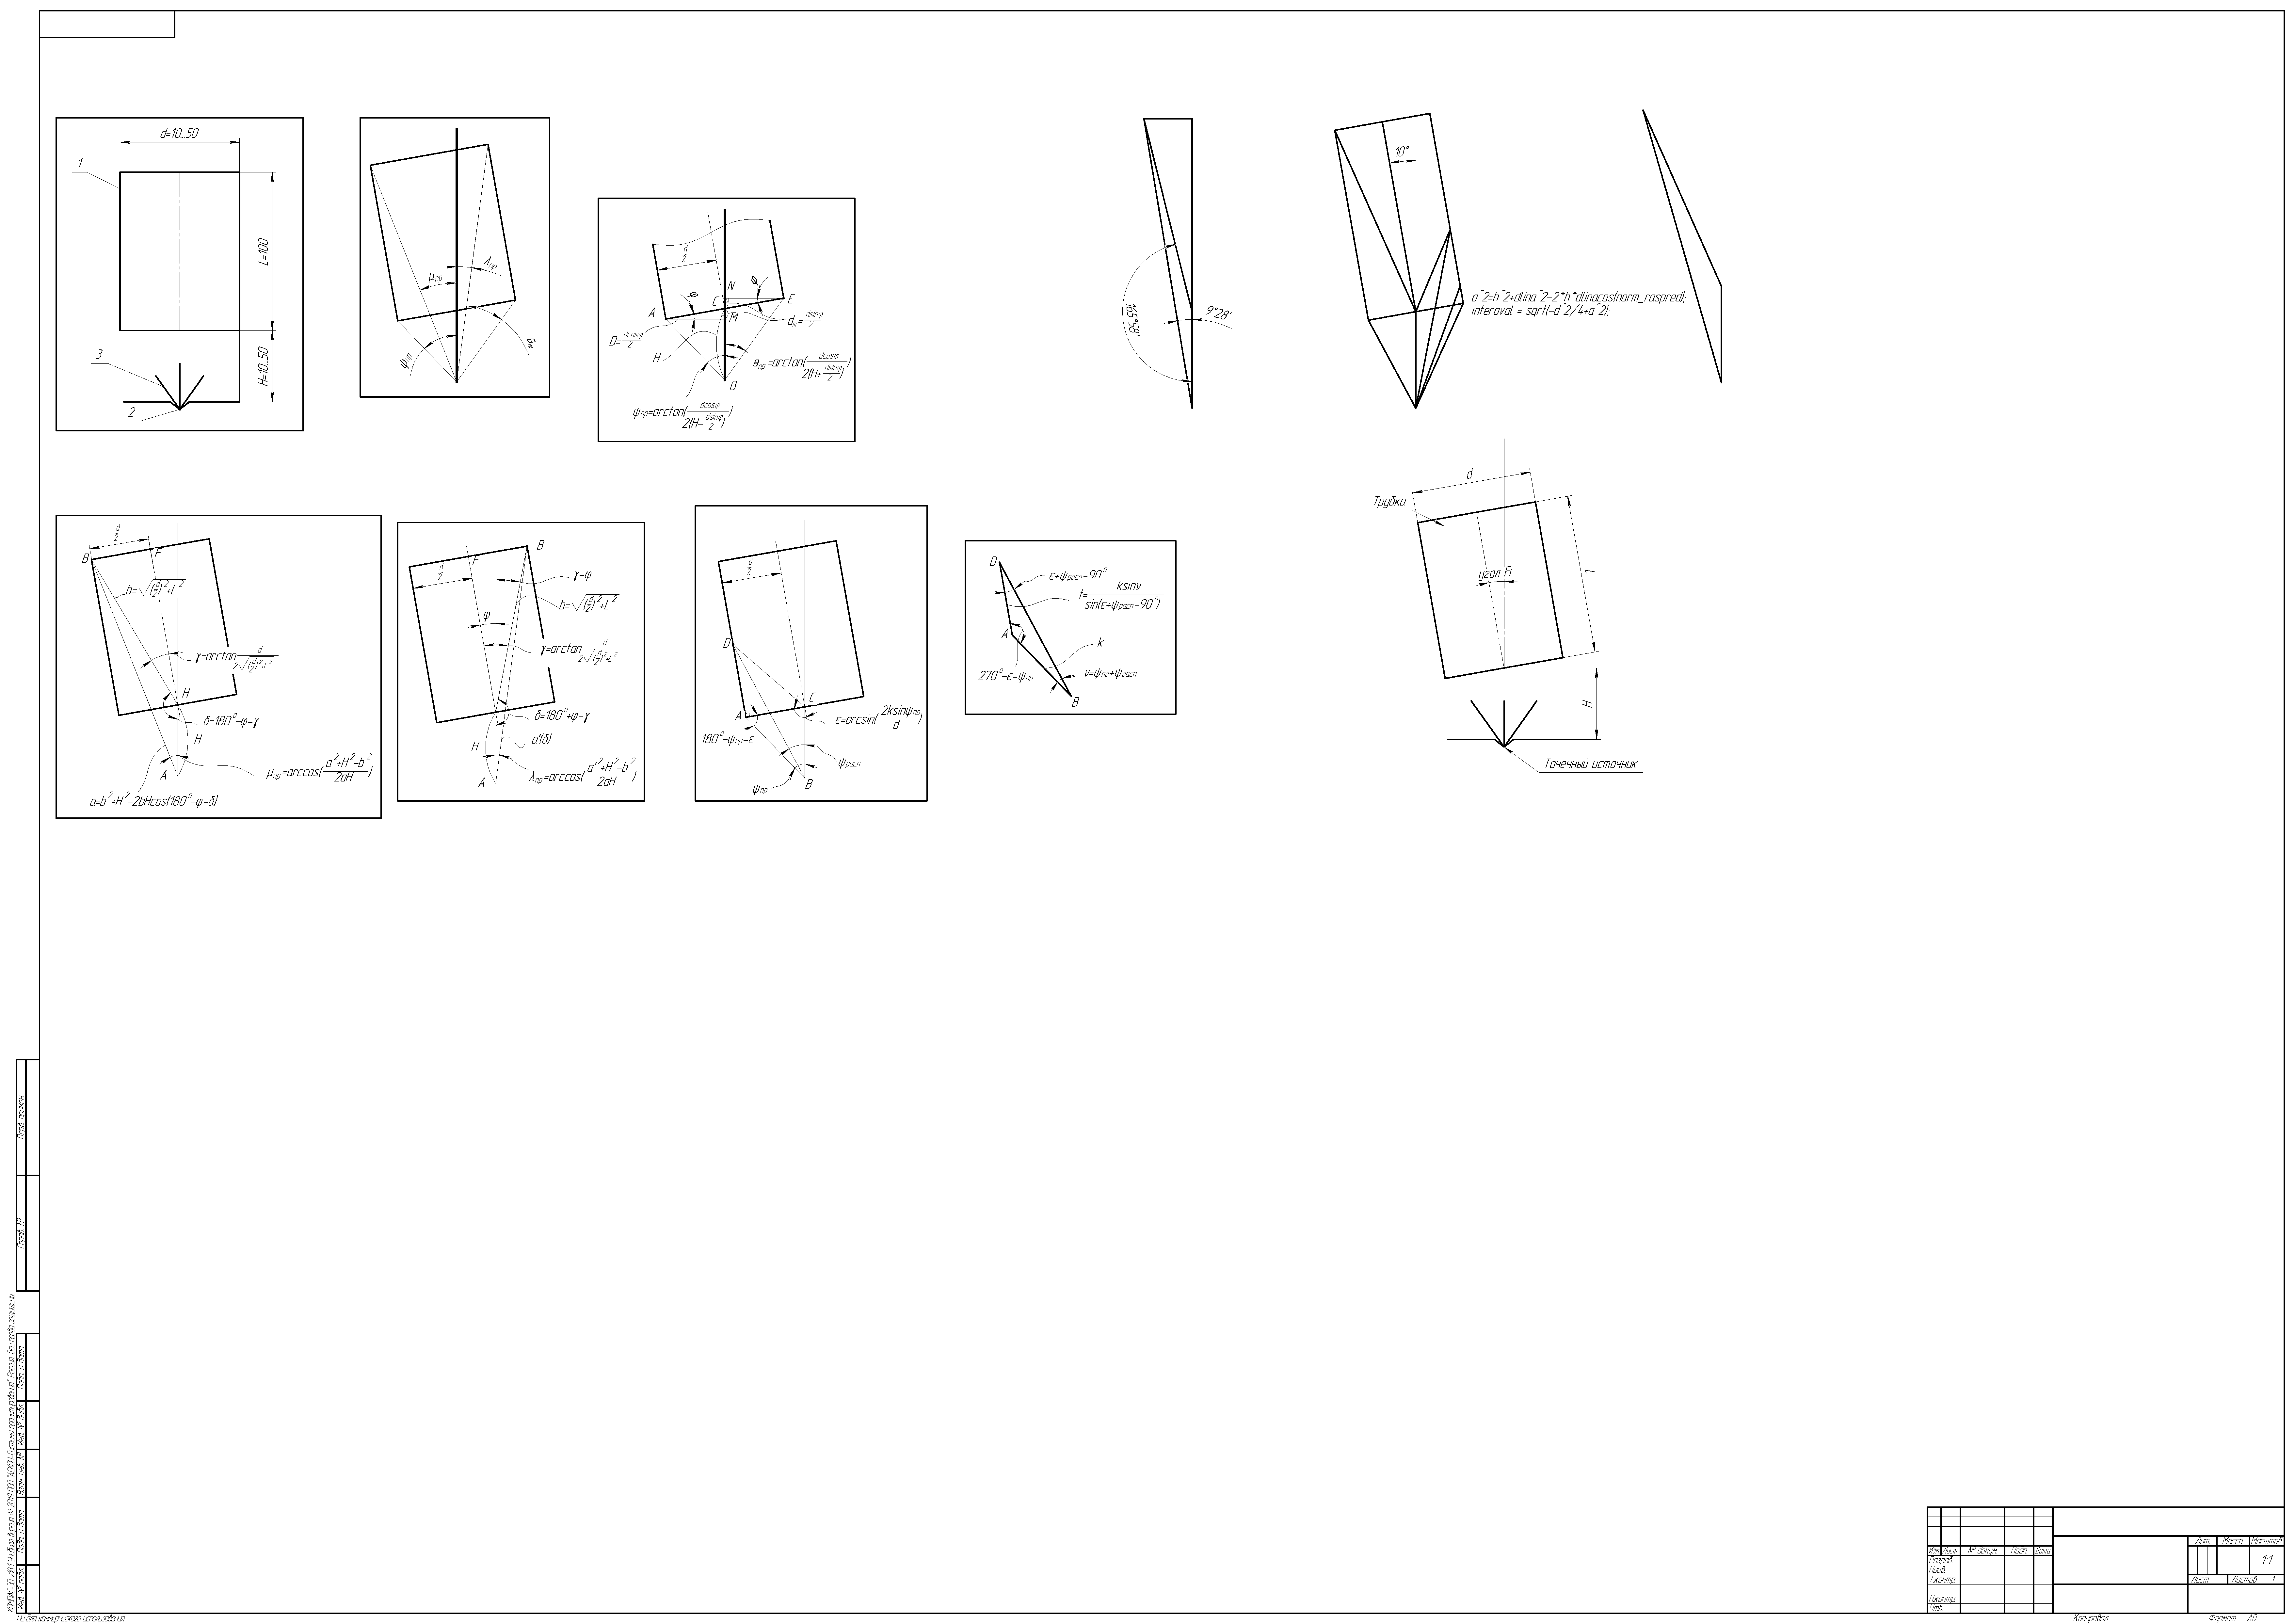
\includegraphics[trim=1030 1215 2015 770, clip, height=0.85\linewidth]{../images/schemes}
		\caption{Вычисление координаты молекулы}
		\label{fig:calculate}
	\end{subfigure}
	\begin{subfigure}{0.5\linewidth}
		\centering
		%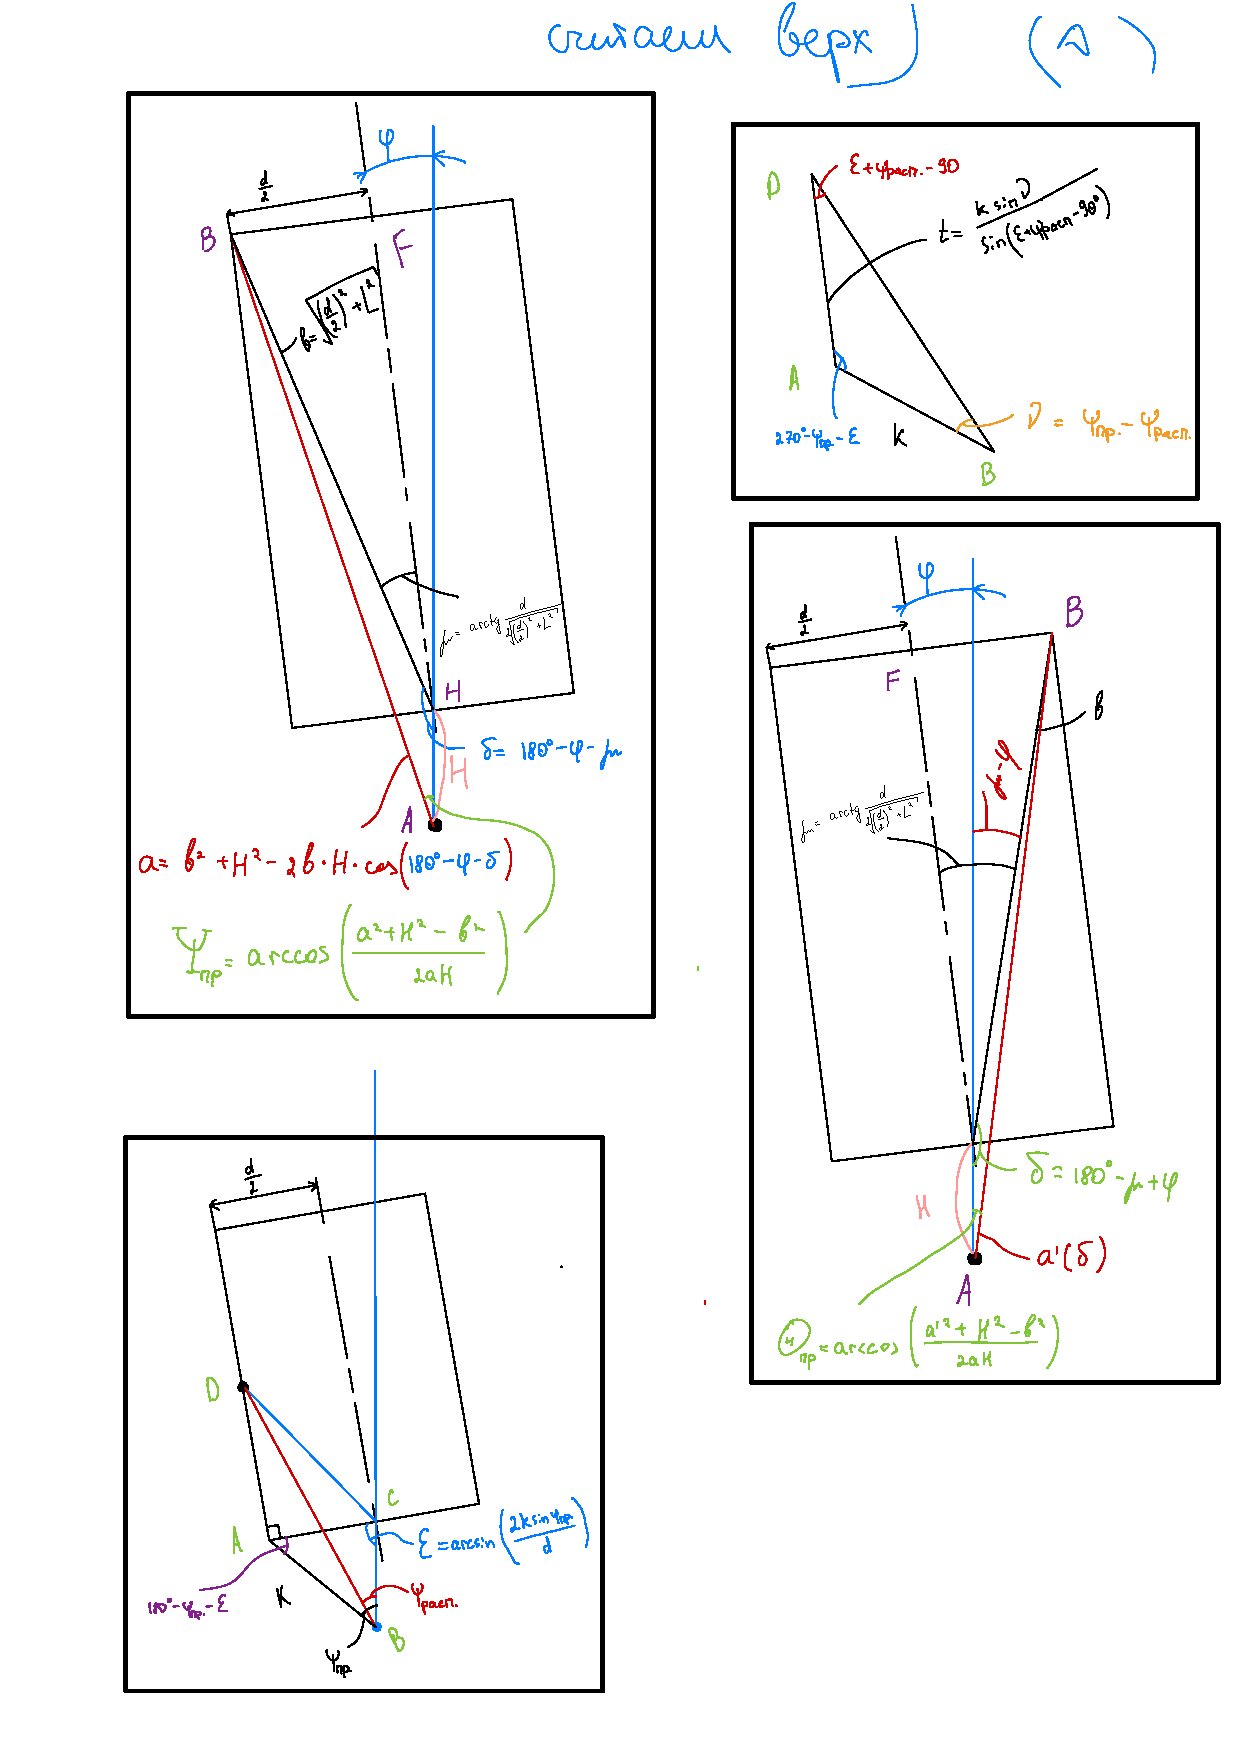
\includegraphics[trim=355 610 25 70,clip, height=0.8\linewidth]{../images/t2}
		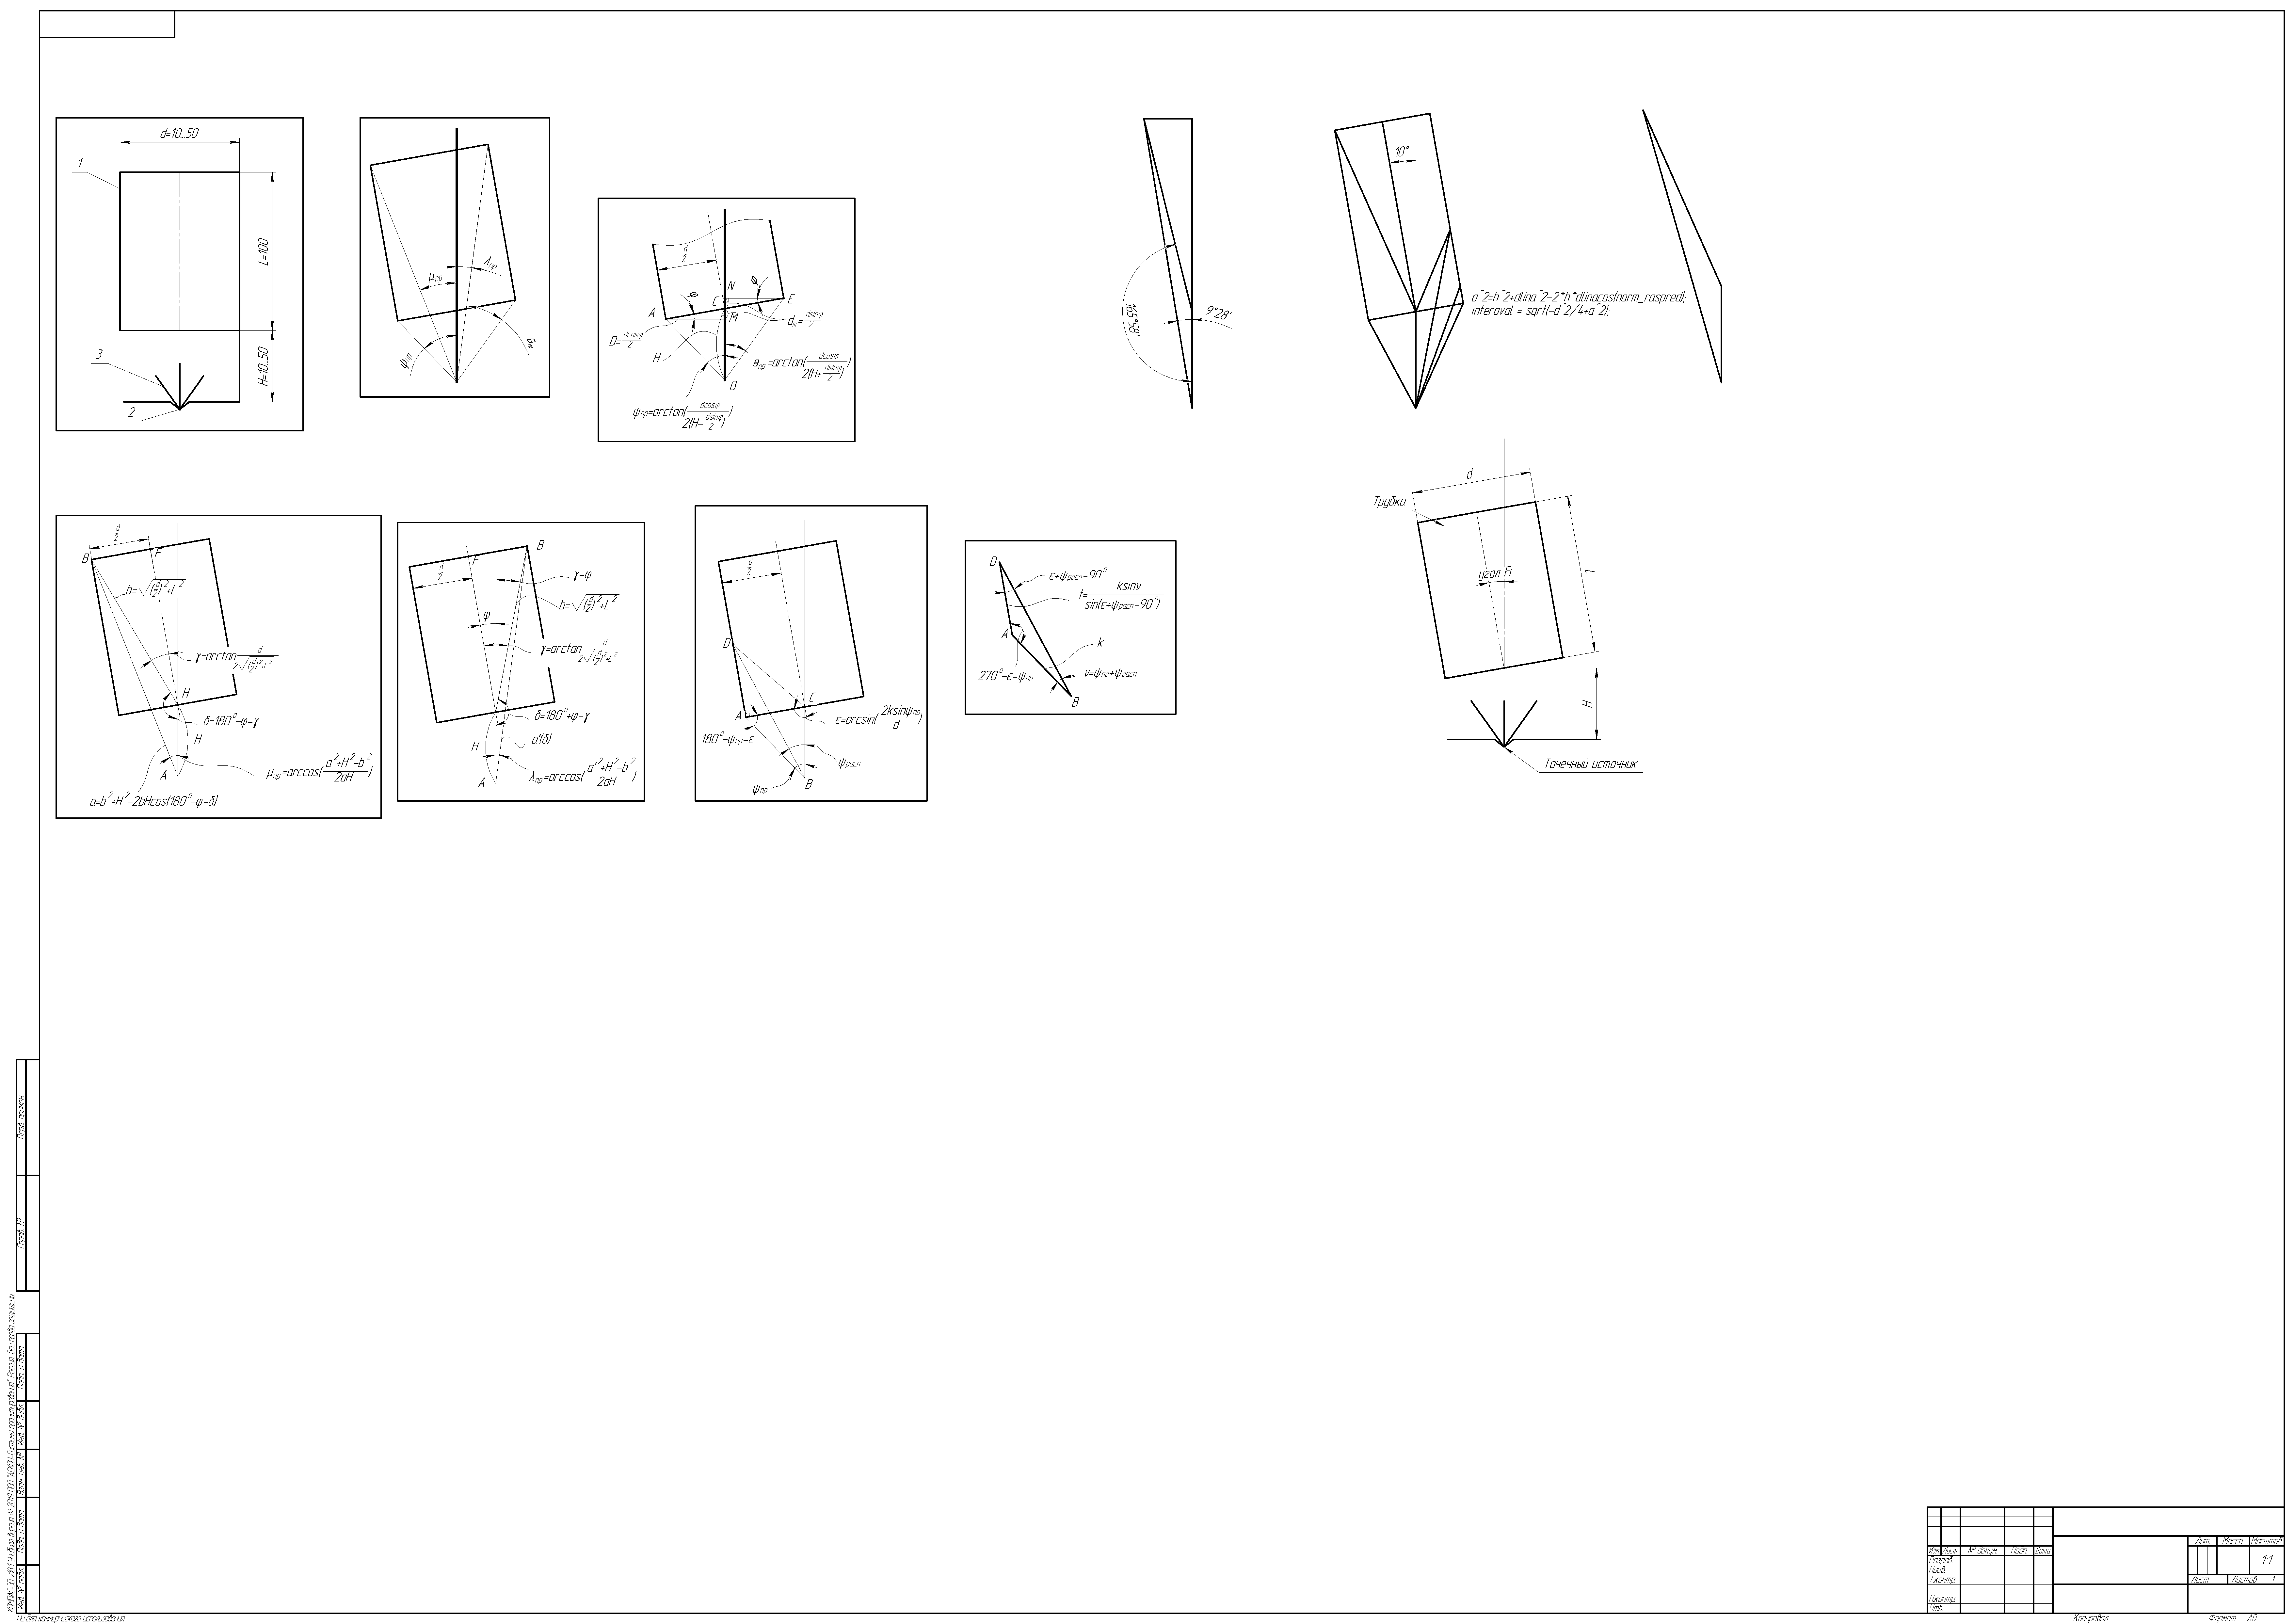
\includegraphics[trim=1425 1345 1660 800, clip, height=0.85\linewidth]{../images/schemes}
		\caption{Треугольник BAD}
		\label{fig:BAD}
	\end{subfigure}
	\caption{Расчётная схема вычисления координаты молекулы}
	\label{fig:monte-carlo}
\end{figure}



\subsection{Принцип работы программы}
\subsubsection{Преобразование Бокса-Мюллера}
\textbf{Преобразование Бокса-Мюллера} --  метод моделирования стандартных нормально распределённых случайных величин:
\begin{enumerate}
	\item \label{choise} Выбираются 2 независимые случайные величины, равномерно распределённые на отрезке $\left[-1, 1\right]$:
	\begin{equation}\label{eq:choise}
		x\in\left[-1, 1\right], \quad y\in\left[-1, 1\right]
	\end{equation}
	\item Вычисляем $s$:
	\begin{equation}
		s = x^2+y^2
	\end{equation}
	\item Если 
	\begin{equation}
		0<s\leq 1
	\end{equation}
	то вычисляем $z_0$ и $z_1$:
	\begin{aleq}
		z_0 &= x\sqrt{\frac{-2\ln s}{s}}\\
		z_1 &= y\sqrt{\frac{-2\ln s}{s}}
	\end{aleq}
	в противном случае повторяем пункт \rbf{choise} и уравнение \eqref{eq:choise}.
\end{enumerate}

В листинге \rbf{list:box_mueller} приведена реализация алгоритма Бокса - Мюллера на языке C++.
\begin{lstlisting}[caption=Реализация алгоритма Бокса-Мюллера,captionpos=b, label={list:box_mueller}]
	double box_muller ()
	{
		double s;
		static quint64 i = 0;
		double x;
		double y;
		double q;
		double w;
		do
		{
			x = randomnum();
			y = -randomnum();
			s = x * x + y * y;
			q = x * qSqrt((-2 * qLn(s))/s);
			w = y * qSqrt((-2 * qLn(s))/s);
		}
		while (s>1 || s==0 || qAbs(q)>1 || qAbs(w) > 1||qAbs(q)>1);
		i++;
		if (i % 2 == 0)
		return w;
		else
		return q;
	}
\end{lstlisting}
\subsubsection{Генерация случайных чисел в библиотеке Qt}
Qt предоставляет класс \textit{QRandomGenerator} для генерации случайных чисел. Функция \textit{randomnum()} из листинга \rbf{list:box_mueller} реализовывается как раз при помощи этого класса. Реализация функции приведена в листинге \rbf{list:randomnum}.

\begin{lstlisting}[caption=Генерация случайных чисел,captionpos=b, label={list:randomnum}]
double randomnum()
{
	QRandomGenerator generator;
	return generator.global()->generateDouble();
}
\end{lstlisting}
\subsubsection{Реализация программы на языке C++}	
Первым делом задаются начальные значения. Было принято, что расстояние от источника до центра основания $H$, угол наклона оси трубки $\phi$ и её диаметр $d$ лежат в следующих интервалах:
\begin{aleq}
	H &\in \left[10, 50\right]\text{мм}\\
	\phi &\in \left[0, 10\right]\grad\\
	d &\in \left[10, 50\right]\text{мм}
\end{aleq}


\begin{lstlisting}[caption=Исходные значения,captionpos=b, label={list:initval}]
	double H = 30;
	double L = 100;
	double fi_pi = 5;//tut
	double fi = fi_pi*M_PI/180;
	double d = 40;//tut
	double r = 145e-12;
\end{lstlisting}

Затем вычисляются величины по формулам, указанным в \refpar{par:geom}.

\begin{lstlisting}[caption=Вычисление граничных условий,captionpos=b, label={list:calculate}]
	double left_down_angle = qAtan(d*qCos(fi)/(2*(H-d/2*qSin(fi))));
	double right_down_angle = qAtan(d*qCos(fi)/(2*(H+d/2*qSin(fi))));
	double left_down_dlina = d*qCos(fi)/(2*(qSin(left_down_angle)));
	double right_down_dlina = d*qCos(fi)/(2*(qSin(right_down_angle)));
	double left_up_dlina = sqrt(pow(d/2,2)+pow(L,2)+pow(H,2)-2*sqrt(pow(d,2)/4+pow(L,2))*H*qCos(M_PI-fi-qAtan(d/(2*L))));
	double left_up_angle = qAcos(-(pow(d,2)/4+pow(L,2)-pow(left_up_dlina,2)-pow(H,2))/(2*H*left_up_dlina));
	double right_up_dlina = sqrt(pow(d/2,2)+pow(L,2)+pow(H,2)-2*sqrt(pow(d,2)/4+pow(L,2))*H*qCos(M_PI+fi-qAtan(d/(2*L))));
	double right_up_angle = qAcos(-(pow(d,2)/4+pow(L,2)-pow(right_up_dlina,2)-pow(H,2))/(2*H*double left_down_dlina = d*qCos(fi)/(2*(qSin(left_down_angle)));
	double right_down_dlina = d*qCos(fi)/(2*(qSin(right_down_angle)));
	qDebug() << right_down_dlina << "right_down_dlina";
	double left_up_dlina = sqrt(pow(d/2,2)+pow(L,2)+pow(H,2)-2*sqrt(pow(d,2)/4+pow(L,2))*H*qCos(M_PI-fi-qAtan(d/(2*L))));
	double left_up_angle = qAcos(-(pow(d,2)/4+pow(L,2)-pow(left_up_dlina,2)-pow(H,2))/(2*H*left_up_dlina));
	double right_up_dlina = sqrt(pow(d/2,2)+pow(L,2)+pow(H,2)-2*sqrt(pow(d,2)/4+pow(L,2))*H*qCos(M_PI+fi-qAtan(d/(2*L))));
	double right_up_angle = qAcos(-(pow(d,2)/4+pow(L,2)-pow(right_up_dlina,2)-pow(H,2))/(2*H*right_up_dlina));_up_dlina));
	double eps_left = qAsin(left_down_dlina*2*qSin(left_down_angle)/d);
	double eps_right = M_PI-eps_left;
\end{lstlisting}

Далее начинается цикл из десяти миллионов итераций (листинг \rbf{list:main}). Именно здесь реализуются алгоритмы, описанные выше.

\begin{lstlisting}[caption=Тело программы,captionpos=b, label={list:main}]
	for (int j = 0; j < 10000000; ++j)
	{
		double buff = box_muller();
		if (j%1000000 == 0)
		qDebug() << j/1000000 <<"/10";
		if (qAsin(buff)>-right_down_angle && qAsin(buff)<-right_up_angle)
		{
			double rh = dlina(right_down_angle,right_down_dlina,eps_right,qAsin(qAbs(buff)));
			right_values[address(rh)].i++;
			right_values[address(rh)].vec.push_back(rh);
		}
		else if (qAsin(buff)<left_down_angle && qAsin(buff)>left_up_angle)
		{
			double lh = dlina(left_down_angle,left_down_dlina,eps_left,qAsin(buff));
			left_values[address(lh)].i++;
			left_values[address(lh)].vec.push_back(lh);
		}
	}
\end{lstlisting}

После исполнения программы данные из массивов записываются в файл (см. листинг \rbf{list:file}):
\begin{lstlisting}[caption=Запись данных в файл,captionpos=b, label={list:file}]
	QFile left_file(filename);
	QTextStream left_data(&left_file);
	for (const auto& amount:left_values) {
		left_data << amount.second.i*2*r*pow(10,6)/10 << "\n";
	}
	left_data<< "sep" << "\n"<<"\n";
	for (const auto& amount:right_values) {
		left_data << amount.second.i*2*r*pow(10,6)/10 << "\n";
	}
	left_file.close();
\end{lstlisting}

\end{document}